\documentclass{article}
\usepackage{amsmath}
\usepackage{xeCJK}
\usepackage{amssymb}
\usepackage{geometry}
\geometry{left=3.0cm, right=3.0cm, top=3.5cm, bottom=2.5cm}
\setlength{\parindent}{0pt}
\renewcommand{\baselinestretch}{1.65}
\newcommand\chfrac[2]{\frac{\;#1\;}{\;#2\;}}
\makeatletter
\renewcommand*\env@matrix[1][\arraystretch]{%
  \edef\arraystretch{#1}%
  \hskip -\arraycolsep
  \let\@ifnextchar\new@ifnextchar
  \array{*\c@MaxMatrixCols c}}
\makeatother
\usepackage{arydshln}
\usepackage{galois}
\usepackage{mathrsfs}
\usepackage{amssymb}
\usepackage{tikz}
\usetikzlibrary{backgrounds}
\usetikzlibrary{arrows}
\usetikzlibrary{plotmarks}
\usetikzlibrary{scopes}


\title{数理泛函分析与复变函数试卷及参考解答}
\author{@慕水 \\ 不对解答的正确性做任何的保证}
\date{最近更新: 2017年7月5日}


\begin{document}
\maketitle
\section{2011-2012学年第二学期泛函分析期末考试(09级)}
\textbf{一、(本题40分, 每小题8分) 证明以下结论:}  \\

(1) 设$E$是$\mathbb{K}$中的闭集, 则$A = \{ x=(x_1, x_2, \cdots) \in l^p: x_i \in E (\forall i) \}$ 是$l^p \  (1 \leq p < \infty)$中的闭集. 

\textbf{证明:} 

设$ \{x^{(n)}_i \} \subset A$, 且$ x^{(n)} = (x^{(n)}_1, x^{(n)}_2, \cdots) \rightarrow x = (x_1, x_2, \cdots)$. 下证明$x^{(n)}_i \rightarrow x_i$ 且 $x \in A$. 

由于$x^{(n)} \rightarrow x$, 所以, $\forall \epsilon >0, \exists N>0$, 当$n > N$, 有:
$$ \Vert{x - x^{(n)} }\Vert = ( \sum\limits_{i=1}^{\infty} |x_i - x^{(n)}_i|^p )^{\frac{1}{p}} < \epsilon \ \ \ \ (1) $$
所以:
$$ |x_i - x^{(n)}_i| \leq ( \sum\limits_{i=1}^{\infty} |x_i - x^{(n)}_i|^p)^{\frac{1}{p}} < \epsilon $$
即: $x^{(n)}_i \rightarrow x_i$. 由于$E$是闭集, 则有$x_i \in E$. 下证明: $x \in A$. 由(1)式可知:
$$ \sum\limits_{i=1}^{\infty} |x_i - x^{(n)}_i|^p < \epsilon^p < +\infty$$
所以, $x-x^{(n)} \in l^p$. 由于$l^p$是线性空间, 所以$x = x - x^{(n)} + x^{(n)} \in l^p$.

综上, $x \in A$. 即:$A$是$l^p$中的闭集. \\  \\


(2) 当$|\lambda| < (e-1)^{-1}$时, $L^2[0,1]$上的算子$(Tx)(t) = \lambda \int_0^1 \sqrt{e^{s+t}}x(s)ds$存在唯一的不动点. 

\textbf{证明:} 

作映射$T: L^2[0,1] \rightarrow L^2[0,1]$,
$$ (Tx)(t) = \lambda \int_0^1 \sqrt{e^{s+t}}x(s)ds $$
对于$\forall x_1(t), x_2(t) \in L^2[0,1]$, 由Holder不等式可得:
\begin{align*}
\Vert Tx_1 - Tx_2 \Vert_2^2 &= \int_0^1|\lambda \int_0^1 \sqrt{e^{s+t}}x_1(s)ds - \lambda \int_0^1 \sqrt{e^{s+t}}x_2(s)ds|^2 dt \\
 & = |\lambda|^2 \int_0^1|\int_0^1 \sqrt{e^{s+t}}(x_1(s) - x_2(s))ds|^2 dt \\
 & \leq |\lambda|^2 (\int_0^1 |x_1(s) - x_2(s)|^2ds)^{\frac{1}{2}}(\int_0^1 (\int_0^1 e^{s+t}ds)^{\frac{1}{2}}dt)  \\
 & = (e-1)^2|\lambda|^2 \Vert x_1 - x_2 \Vert_2^2
\end{align*}
由于$|\lambda| < (e-1)^{\frac{1}{2}}$, 所以$(e-1)^2|\lambda|^2 < 1$, 所以映射$T$是压缩的.

由于$L^2[0,1]$是完备距离空间, 由压缩映射原理可知, 算子$T$存在唯一的不动点. \\  \\


(3) 设$A$是距离空间$X$中的紧集, $x \in X$, 则必存在$y_0 \in A$使得$d(x, y_0) = \inf\limits_{y \in A} d(x,y)$. 

\textbf{证明:}

对于$x \in X$, 定义函数$f:$ $f(y) = d(x, y), y \in A$. 下证明$f$是$A$上的连续函数.
注意到:
$$ d(x,z) \leq d(x,y) + d(y,z)  \ \ \ \ \Rightarrow \ \ \ \ d(x,z) - d(x,y) \leq d(y,z) $$
$$ d(x,y) \leq d(x,z) + d(y,z)  \ \ \ \ \Rightarrow \ \ \  d(x,z) - d(x,y) \leq -d(y,z)$$
所以$|d(x,z) - d(x,y)| \leq d(y,z)$. 所以有:
$$ |f(y_1) - f(y_1)| = |d(x,y_1) - d(x,y_2)| \leq d(y_1, y_2) $$
从而$\forall \epsilon >0, \exists \delta = \epsilon$, 当$d(y_1, y_2) < \delta$, 有$|f(y_1) - f(y_2)| < \epsilon$. 

所以$f$在$A$上连续. 又由于$A$是紧集, 所以, $\exists y_0 \in A$, 使得:
$$ d(x, y_0) = f_{min}(y) = \inf\limits_{y \in A} d(x,y) $$  \\  \\ 



(4) 设$a_n = \text{ln}(1+\dfrac{1}{n})(n \geq 1)$. 则$l^1$上算子$T(x_1, x_2, \cdots) = (a_1x_1, a_2x_2, \cdots)$是紧算子. 

\textbf{证明:} 

记$x = (x_1, x_2, \cdots)$, 则:
$$\Vert Tx \Vert_1 = \sum\limits_{n=1}^{\infty} |a_nx_n| \leq \sup\limits_{n \geq 1} |a_n| \sum\limits_{n=1}^{\infty} |x_n| = (\sum\limits_{n=1}^{\infty} |x_n|)\text{ln}2 $$
易验证$T$是线性的. 所以$T$是有界线性算子.对每个$n=1,2,\cdots$, 令:
$$ T_n(x_1, x_2, \cdots) = (a_1x_1, a_2x_2, \cdots, a_nx_n) $$
则每个$T_n$是有界的有限秩算子, 从而每个$T_n$是紧算子. 对于$\forall x=(x_i) \in l^1$, 有:

$$ \Vert Tx - Tx_n \Vert_1 = \sum\limits_{k=n+1}^{\infty} |a_kx_k| \leq (\sup\limits_{k \geq n+1} |a_k|) \sum\limits_{k=n+1}^{\infty} |x_k| \leq (\sup\limits_{k \geq n+1} |a_k|) \sum\limits_{n=1}^{\infty} |x_n| = \Vert x \Vert_1 \text{ln}(1+\frac{1}{n+1}) $$
所以:
$$ \Vert T - T_n \Vert \leq \text{ln}(1+\frac{1}{n+1}) \rightarrow 0 \ \ (n \rightarrow \infty) $$
所以, $T$是紧算子. \\  \\ 


(5) 设$E = \{ f \in L^2(-\infty, +\infty): \text{在}(-\infty, 0] \ \text{上} f=0 \  a.e. \}$. 求$E^{\perp}$. 

\textbf{解:}

任取$g \in E^{\perp}$, 则对于$\forall f \in E$, 有:
$$ (f, g) = \int_{\mathbb{R}} f \overline{g} dx = \int_{-\infty}^0 f \overline{g}dx + \int_{0}^{+\infty} f\overline{g}dx $$
由于在$(-\infty, 0]$上$f = 0\ a.e. $, 则存在$m(E)=0$, 当$x \in (-\infty, 0] \setminus E, f=0$. 

则当$x \in (-\infty, 0] \setminus E$时, $f\overline{g} =0$. 即存在$E_1, m(E_1) \leq m(E) =0$, 使得当$x \in (-\infty, 0] \setminus E_1$时, 
$$fg=0$$
 即: 
$$   f\overline{g} = 0\ a.e. \ \ \ \ x\in (-\infty, 0]$$
所以可得:
$$ \int_{-\infty}^0 f\overline{g} dx = 0 $$
由$f$的任意性, 取$f = g, \ x \in (0, \infty)$, 则:
$$ (f,g) =\int_{-\infty}^0 f \overline{g}dx + \int_{0}^{+\infty} f\overline{g}dx = \int_{0}^{+\infty} |g|^2 dx = 0  $$
当$g = 0 \ a.e. \ x \in [0, \infty)$时, 上式成立. 假设$ g = 0 \ a.e. \ x \in [0, +\infty)$不成立. 

则存在可测集$E_2, m(E_2) >0$,当$x \in E_2$时, $|g| >0$.从而:
$$ (f, g)= \int_{0}^{+\infty} |g|^2 dx > \int_{E_2} |g|^2 dx>0$$
矛盾. 所以:$g=0 \ a.e. \ x \in [0, +\infty)$. 由于$g$是从$E^{\perp}$中任意取的元素, 所以:
$$ E^{\perp} = \{ g \in L^2(-\infty, +\infty): \text{在}[0,+\infty) \ \text{上} g=0 \  a.e. \} $$ \\ 

\textbf{以下六题任选五题,每题12分}

\textbf{二、} 设$C^{(1)}[a,b]$是$[a,b]$上具有连续导数函数的全体. 在$C^{(1)}[a, b]$上定义:
$$ \Vert{x}\Vert = \max\limits_{a \leq t \leq b} |x(t)| + \max\limits_{a \leq t \leq b}|x'(t)|, \ \ x \in C^{(1)}[a, b]  $$
\hspace{2em} 证明: $C^{(1)}[a, b]$是完备的.  

\textbf{证明:}

设$\{x_n \}$是$C^{(1)}[a, b]$中的Cauchy列, 则$\forall \epsilon >0, \exists N>0$, 当$m,n >N$, 有:
$$ \Vert x_m - x_n \Vert = \max\limits_{a \leq t \leq b} |x_m(t) - x_n(t)| + \max\limits_{a \leq t \leq b}|x_m^{'}(t) - x_n^{'}(t)| $$
所以可得:
$$ \max\limits_{a \leq t \leq b} |x_m(t) - x_n(t)|, \ \  \max\limits_{a \leq t \leq b}|x_m^{'}(t) - x_n^{'}(t)| < \epsilon $$
即:$x_(t), x_n^{'}(t)$都是一致收敛的.记:$x_n \rightarrow x, x_n^{'} \rightarrow x^{(')}$. 由一致收敛函数列可微性质可得:
$$ x'(t) = \dfrac{\text{d}}{\text{d}x} (\lim\limits_{n \rightarrow \infty} x^{n}(t)) = \lim\limits_{n \rightarrow \infty} x_n^{'} = x^{(')}  $$
而$x_n(t)$的连续性再结合$x_n(t)$的一致收敛性可导出$x(t)$的连续性, 而$x_n^{'}(t)$的连续性以及一致收敛性可以导出$x^{(')}(t)$的连续性.

所以$x(t)$具有连续的导数, $x(t) \in C^{(1)}[a,b]$. 所以$C^{(1)}[a,b]$是完备的.  \\  \\



\textbf{三、} 计算$C[-\pi, \pi]$上的线性泛函$f(x) = \int_{-\pi}^{\pi}x(t)sintdt$的范数. 

\textbf{证明:}

首先, 有:
$$ |f(x)| = |\int_{-\pi}^{\pi} x(t)sint dt| \leq \int_{-\pi}^{\pi} |x(t)sint|dt \leq (\max\limits_{a \leq t \leq b} |x(t)|) \int_{-\pi}^{\pi} |sint|dt = (\int_{-\pi}^{\pi} |sint|dt) \Vert x \Vert$$
所以, $\Vert f \Vert \leq \int_{-\pi}^{\pi} |sint|dt = 4 $. 另一方面, 令:
$$x_0(t) = \left\{
\begin{array}{lcl}
-1  &, & t \in [-\pi, -\epsilon] \\
\dfrac{x}{\epsilon} &, & t \in (-\epsilon, \epsilon) \\
1   &, & t \in [\epsilon, \pi]
\end{array} \right.
$$
则$x_0 \in C[-\pi, \pi]$且$\Vert x \Vert = 1$, 于是有:
\begin{align*}
f(x_0) &= \int_{-\pi}^{\pi} x_0(t)sintdt \\
       &= \int_{-\pi}^{-\epsilon} (-sint)dt + \int_{-\epsilon}^{\epsilon} \dfrac{tsint}{\epsilon} dt + \int_{\epsilon}^{\pi} sintdt  \\
       &> cos(\epsilon)+1 + 1 + cos(\epsilon)= 4-4sin^2(\dfrac{\epsilon}{2}) \\
       &> 4-\epsilon^2
\end{align*}
所以$\Vert f \Vert > 4 - \epsilon^2$. 由$\epsilon$的任意性可知, $\Vert f \Vert \geq 4$.综上, $\Vert f \Vert = 4$. \\  \\

\textbf{四、} (1) 设$X, Y$是距离空间, 若$T: X \rightarrow Y$是双射的闭算子, 则$T^{-1}$是闭算子. 

\hspace{2em} (2) 用闭图像定理证明逆算子定理.   

\textbf{证明:} 

(1) 设 $\{y_n \} \subset Y$, 且$y_n \rightarrow y, T^{-1}y_n \rightarrow x$. 

\hspace{1.5em} 由于$T$是双射, 所以存在唯一的$x_n \in X$, 使得$x_n = T^{-1}y_n$. 所以$Tx_n = T(T^{-1}yn) = y_n \rightarrow y$.

\hspace{1.5em} 由于$T$是闭算子, 所以 $y = Tx$, 从而$x = T^{-1}y$. 所以$T^{-1}$是闭算子. \\

(2) 设$X, Y$是Banach空间, $T$是双射且有界的线性算子.

\hspace{1.5em} 线性算子$T$有界 $\Leftrightarrow$ $T$连续 $\Rightarrow$ $T$是闭算子.

\hspace{1.5em} 由(1)可知, $T^{-1}$是闭算子. 再由闭图像定理, $T^{-1}$有界, 得证.  \\  \ 


\textbf{五、} 设$X$是赋范空间, $\{ x_n \}$ 是$X$中的有界序列, $x \in X$. 证明若对$X^*$的某个稠密子集$A$中的每个

\hspace{2em} 元$f$, 成立$f(x_n) \rightarrow f(x)$, 则$x_n \xrightarrow{w} x$. 

\textbf{证明:}

对于$\forall f \in X^*$, 由于$A$在$X$中稠密, 所以$\exists f_n \in A$, 使得:
$$ f_n \rightarrow f $$
由于$\{ x_n \}$是有界序列, 所以$\forall x \in \{ x_n \}$,当$k>N$, 有
$$|f_k(x) - f(x)| \leq \Vert f_k - f \Vert \Vert x \Vert < \dfrac{\epsilon}{3}$$
 由题目条件可知:
$$ f_k(x_n) \rightarrow f_k(x) \ \ \ \Rightarrow \ \ \ |f_k(x_n) - f_k(x)| < \dfrac{\epsilon}{3}, \ \ k=1,2, \cdots $$
所以$\forall f \in X^*$, 有:
\begin{align*}
|f(x_n) - f(x)| &= |f(x_n) - f_n(x_n) + f_n(x_n) -f_n(x) + f_n(x) - f(x) | \\
                &\leq |f(x_n) - f_k(x_n)| + |f_k(x_n) - f_k(x)| + |f_k(x) - f(x)|  \\
                &< \dfrac{\epsilon}{3} + \dfrac{\epsilon}{3} + \dfrac{\epsilon}{3} \\
                &< \epsilon
\end{align*}
所以$\forall f \in X^*$, 有$f(x_n) \rightarrow f(x)$. 所以:$x_n \xrightarrow{w} x$. \\  \\


\textbf{六、} 证明$(R^n, \Vert \cdot \Vert_1)^* \cong (R^n, \Vert \cdot \Vert_{\infty}) $, 其中
$$ \Vert x \Vert_1 = \sum\limits_{i=1}^n |x_i|, \ \ \Vert x \Vert_{\infty} = \max\limits_{1 \leq i \leq n} |x_i|, \ \ x=(x_1, \cdots, x_n) \in R^n $$ 

\textbf{证明:} 

分三个步骤证明上述命题.

(1) 设$\{e_i \}_{i=1}^n$是$R^n$中的标准基. 对于$\forall f \in R^n, \Vert \cdot \Vert_1)^*$. 令$a_i = f(e_i)(i=1, 2, \cdots)$. 

对于$\forall x=(x_1, x_2, \cdots, x_n)$, 有:
$$ f(x) = f(\sum\limits_{i=1}^n x_ie_i) = \sum\limits_{i=1}^n x_if(e_i) = \sum\limits_{i=1}^n a_ix_i $$
这表明$\forall f \in \forall f \in R^n, \Vert \cdot \Vert_1)^* $, $f$的一般表达式为$f =\sum\limits_{i=1}^n a_ix_i$.

对每个$i=1,2,\cdots$, 有:
$$ |a_i| = |f(e_i)| \leq \Vert f \Vert \Vert e_i \Vert_1 = \Vert f \Vert $$
所以, $(\max\limits_{n \geq 1} |a_n|) \leq \Vert f \Vert$. 记$a=(a_1, a_2, \cdots, a_n)$,从而: $a \in (R^n, \Vert \cdot \Vert_{\infty})$. \\

(2)反过来, 对$\forall a = (a_1, a_2, \cdots, a_n) \in (R^n, \Vert \cdot \Vert_{\infty})$, 令:
$$ f(x) = \sum\limits_{i=1}^n a_ix_i, \ \ x=(x_1, x_2, \cdots, x_n) \in (R^n, \Vert \cdot \Vert_1) $$
则$f$是$(R^n, \Vert \cdot \Vert_1)^*$上的线性泛函, 且$f(e_i) = a_i$. 对$\forall x = (x_1, \cdots, x_n) \in (R^n, \Vert \cdot \Vert_1)$:
$$ |f(x)| = |\sum\limits_{i=1}^n a_ix_i| \leq (\max\limits_{k \geq 1} |a_k|) \sum\limits_{i=1}^n |x_i| = \Vert a \Vert_{\infty} \Vert x \Vert_1 $$
这说明, $\Vert f \Vert \leq \Vert a \Vert_{\infty}$. \\

(3)作映射:
\begin{center}
\begin{tabular}{cccc}
 $T:$  &  $(R^n, \Vert \cdot \Vert_1)^*$ & $\rightarrow$ & $(R^n, \Vert \cdot \Vert_{\infty})$ \\
       &                 $f$            &  $\mapsto$   &  $a =(a_1, a_2, \cdots, a_n)$ \\
\end{tabular}
\end{center}
易知$T$是线性映射. 由(2)知$T$是满射. 且:
$$ \Vert Tf \Vert_{\infty} = \Vert a \Vert_{\infty} = \Vert f \Vert$$
所以$T$是保距同构映射. 从而: $(R^n, \Vert \cdot \Vert_1)^* \cong (R^n, \Vert \cdot \Vert_{\infty}) $.  \\  \\ 


\textbf{七、} 设$\lambda_1, \cdots, \lambda_n \in \mathbb{K}$. 定义$T: l^2 \rightarrow l^2, T(x_1, x_2, \cdots) = (\lambda_1x_1, \cdots, \lambda_nx_n, 0, \cdots)$. 

\hspace{2em} (1) 求$T$的伴随算子$T^*$的表达式. 

\hspace{2em} (2) 当$\lambda_1, \cdots, \lambda_n$满足什么条件时, $T$是投影算子?  

\textbf{证明:} 

(1) 对于$\forall x=(x_1, x_2, \cdots) \in l^2$, 
$$ \Vert Tx \Vert_2 = (\sum\limits_{k=1}^n |\lambda_i x_i|^2)^{\frac{1}{2}} \leq (\sup\limits_{k \geq 1} \lambda_i) (\sum\limits_{i=1}^n |x_i|^2)^{\frac{1}{2}} \leq  (\sup\limits_{k \geq 1} \lambda_i) \Vert x \Vert_2 $$
易验证, $T$是线性算子. 所以, $T$是有界线性算子. 设$T^*(y_1, y_2, \cdots) = (z_1, z_2, \cdots)$, 则:$\forall x, y \in l^2$, 有
$$ (Tx, y) = \sum\limits_{i=1}^n \lambda_ix_i\bar{y}_i, \ \ \ (x, T^*y ) = \sum\limits_{i=1}^{\infty} x_i \bar{z_i}$$
依次取$x=e_i=(0,\cdots, 1, 0, \cdots)$, 可以得到: $z_i = \bar{\lambda}_iy_i, (\ i=1,\cdots,n), \ z_i=0, (i \geq n+1)$ 即:
$$ T^*(y_1, y_2, \cdots) = (\bar{\lambda}_1y_1, \bar{\lambda}_2y_2, \cdots, \bar{\lambda}_ny_n, 0, 0, \cdots) $$ 

(2)由于$T$是投影算子当且仅当$T$是幂等和自伴的. 所以, $\forall x \in l^2$,
$$ T(T(x)) = T(\lambda_1x_1, \lambda_2x_2, \cdots, \lambda_nx_n, 0, 0, \cdots) = (\lambda_1^2x_1, \lambda_2^2x_2, \cdots, \lambda_n^2x_n, 0, 0, \cdots) $$
所以, 
$$T^2 = T \ \ \Rightarrow \ \ \lambda_i = \lambda_i^2 \ \ \Rightarrow \ \ \lambda_i = 0, 1 $$
对于自伴性, 
$$ T = T^* \ \ \Rightarrow \ \ \lambda_i = \bar{\lambda}_i \ \ \Rightarrow \ \ \{\lambda_i \}_{i=1}^n\text{是实数列} $$
综上, 当$\lambda_i \in \{0, 1\}, (i=1,2, \cdots, n)$时, $T$是投影算子. 

\newpage



\section{2012-2013年学年第二学期泛函分析期末考试(10级)}
\textbf{一、(本题40分, 每小题8分) 证明以下结论:}  \\

(1) $A = \{ X\in C[a,b]: \int_a^b x(t)dt=0 \}$是$C[a,b]$中的闭集. 

\textbf{证明:}

取$\{ x_n \} \subset A$, 且$x_n \rightarrow x$. 下证明:$x \in A$.

由于$x_n \rightarrow x$, 所以$\forall \epsilon>0, \exists N>0$, 当$n>N$时:
 $$\max\limits_{ a \leq t \leq b} |x(t) - x_n(t)| < \epsilon$$
所以有:

$$ |\int_a^b x(t)dt| = |\int_a^b x(t) - x_n(t)dt| \leq \int_a^b |x(t) - x_n(t)|dt < (b-a)\epsilon  $$
由$\epsilon$的任意性可得, $\int_a^b x(t) dt =0$. 即:$x \in A$. 所以$A$是闭集. \\  \\  


(2) 当$|\lambda| < \dfrac{\pi}{2}$时, $C[0,1]$上的算子$(Tx)(t) = \lambda \int_0^1x(s)cos\dfrac{\pi}{2}s ds + e^t$存在唯一的不动点. 

\textbf{证明:}

作映射$T: C[0,1] \rightarrow C[0,1]$:
$$ (Tx)(t) = \lambda \int_0^1x(s)cos\dfrac{\pi}{2}s ds + e^t $$
对于$\forall x_1, x_2 \in C[0,1]$, 有:
\begin{align*}
\Vert Tx_1 - Tx_2 \Vert &= \Vert \lambda \int_0^1x_1(s)cos\dfrac{\pi}{2}s ds + e^t - \lambda \int_0^1x_2(s)cos\dfrac{\pi}{2}s ds - e^t  \Vert \\
       &= \max\limits_{0 \leq t \leq 1} (\int_0^1 |\lambda||(x_1(s) - x_2(s))cos\dfrac{\pi}{2}s|ds) \\
       &\leq |\lambda|(\max\limits_{0 \leq s \leq 1}|x_1(s) - x_2(s)|)(\max\limits_{0 \leq t \leq 1} \int_0^1 |cos\dfrac{\pi}{2}s| ds) \\
       &=\dfrac{2|\lambda|}{\pi} \Vert x_1 - x_2 \Vert
\end{align*}
由于$|\lambda| < \dfrac{\pi}{2}$, 所以$\dfrac{2|\lambda|}{\pi} <1$. 所以映射$T$是压缩的. 而$C[0,1]$是完备的,由压缩映射原理可知存在唯一不动点. \\  \\  

(3) 令$A = \{ sin(t+\lambda): \lambda \in \mathbb{R} \}$. 则$A$是$C[0,1]$中的列紧集. 

\textbf{证明:}

对于$\forall x=sin(t+\lambda) \in A$, 有$|sin(t+\lambda)| \leq 1$. 所以函数族$A$是一致有界的.

对于$\forall t \in [0,1]$,由微分中值定理可得:
$$ |x(t_1) - x(t_2)| = |sin(t_1+\lambda) - sin(t_2+\lambda)| = |cos(\xi)||t_1 - t_2| \leq |t_1 - t_2|, \ \ \xi \in [0,1] $$ 
所以$x$满足Lipschitz条件, 从而函数族$A$是等度连续的. 由Arzela-Ascoli定理, $A$是$C[0,1]$中的列紧集. \\  \\



(4) 设$X$和$Y$是两个拓扑同构赋范空间. 若$X$是可分的, 则$Y$也是可分的. 

\textbf{证明:}

由于$X$是可分的, 所以存在可数集$ A = \{a_i \}_{i \geq 1} \subset X$, 使得$A$在$X$中稠密.

由于$X, Y$是拓扑同构的, 所以存在从$X$到$Y$的有界线性双射$T: X \rightarrow Y$, 使得$Tx_n = y_n \in Y$.

显然$B$是$Y$中的可数集, 下证明$B$在$Y$中稠密.对于$\forall \epsilon \in \epsilon, \forall y \in Y$, 考虑邻域$U(y, \epsilon)$. 记$Tx = y$.

由于$T$是有界的, 所以$T$是连续的. 从而$\forall \epsilon >0, \exists \delta >0$, 当$d(x, x_0) < \delta$时, $|y-y_0| < \epsilon $

由于$A$在$X$中稠密, 所以$\exists x_k \in U(x, \delta)$. 由于$d(x, x_k) < \delta$, 所以$d(y,y_k) < \epsilon$.

即$\forall \epsilon >0, \forall y \in Y, \exists y_k \in B $, 使得$ y_k \in U(y, \epsilon)$. 从而$B$是$Y$中的稠密集. 

从而$ B= \{y_i \}_{i \geq 1}$是$Y$中可数的稠密子集. 所以$Y$是可分的. \\  \\

 

(5) 设$\alpha(t)$是有界可测函数, $h$是常数. 在$L^2(-\infty, +\infty)$上定义算子$(Ax)(t) = \alpha(t)x(t+h)$, 求$A$的伴随算子$A^*$的表达式.    

\textbf{解:}

显然算子$A$是线性的, 下证明算子$A$是有界的. 我们有:
\begin{align*}
\Vert Ax \Vert_2 &= (\int_{-\infty}^{+\infty} |\alpha(t)x(t+h)|^2dt)^{\frac{1}{2}} \\
                 &\leq (\max\limits_{t\in \mathbb{R}}|\alpha(t)|) (\int_{-\infty}^{+\infty} |x(t+h)|^2dt)^{\frac{1}{2}} \\
                 &= (\max\limits_{t \in \mathbb{R}}|\alpha(t)|) (\int_{-\infty}^{+\infty} |x(t)|^2dt)^{\frac{1}{2}} \\
                 &= (\max\limits_{t \in \mathbb{R}}|\alpha(t)|) \Vert x \Vert_2 
\end{align*}
由于$\alpha(t)$是有界可测函数, 所以$\Vert A \Vert_2 \leq (\max\limits_{t \in \mathbb{R}}|\alpha(t)|) < \infty$. 即$A$是有界的. 

设$(A^*x)(t) = z(t)$, 下面求$A$的伴随算子$A^*$的表达式. 对于$\forall x, y \in L^2(-\infty, +\infty)$, 有:
$$ (Ax, y) = \int_{-\infty}^{+\infty} \alpha(t)x(t+h)\overline{y(t)} = \int_{-\infty}^{+\infty} \alpha(t-h)x(t)\overline{y(t-h)}dt $$
$$ (x, A^*y) = \int_{-\infty}^{+\infty} x(t)\overline{z(t)}dt $$
所以:
$$ (Ax, y) - (x, A^*y) = \int_{-\infty}^{+\infty} x(t)\overline(\overline{\alpha(t-h)}y(t-h) - z(t)) = 0 $$
由$x(t)$的任意性, 取$x(t) = \overline{\alpha(t-h)}y(t-h) - z(t)$, 可得: $z(t) = \overline{\alpha(t-h)}y(t-h)$.所以: 
$$  (A^*y)(t) = \overline{\alpha(t-h)}y(t-h) $$ \\

\textbf{以下六题任选五题,每题12分}

\textbf{二、} 设$X = \{f=(f_i)_{i \geq 1}: f_i \in L^p[a,b], \text{且} \sup\limits_{i \geq 1} \Vert{f_i}\Vert_p < \infty \}$. 在$X$上定义范数$\Vert{f} \Vert= \sup\limits_{i \geq 1} \Vert{f_i}\Vert_p$. 证明$X$按照这个范数所成的赋范空间是完备的.  

\textbf{证明:}

设$f^{(n)}= (f^{(n)}_i)_{i \geq 1} $是$X$中的Cauchy列, 所以$\forall \epsilon >0, \exists N>0$, 当$m,n > N$,有:
$$ \Vert f^{(m)} - f^{(n)} \Vert = \sup\limits_{i \geq 1}\Vert f^{(m)}_i - f^{(n)}_i \Vert < \epsilon \ \ \ (1)$$
所以, 对每个$i = 1, 2, \cdots$, 有:
$$ \Vert f^{(m)}_i - f^{(n)}_i\Vert \leq \sup\limits_{i \geq 1} \Vert f^{(m)}_i - f^{(n)}_i \Vert < \epsilon $$
所以, 对每个$i=1,2, \cdots$, 有$f^{(n)}_i$收敛. 记: $f^{(n)}_i \rightarrow f_i, \ f = (f_1, f_2, f_3 \cdots)$. 

下证明$f \in X$, 且$f^{(n)} \rightarrow f$. 在(1)式中, 令$m \rightarrow \infty$, 有:
$$ \Vert f - f^{(n)} \Vert = \sup\limits_{i \geq 1}\Vert f_i - f^{(n)}_i \Vert < \epsilon  $$ 
所以$f-f^{(n)} \in X$. 由于$X$是赋范空间, 所以$f = f-f^{(n)} + f^{(n)} \in X$. 且式(1)还表明, $\forall \epsilon >0, \exists N>0$, 当$n > N$时, 有:
$$  \Vert f - f^{(n)} \Vert \sup\limits_{i \geq 1}\Vert f_i - f^{(n)}_i \Vert < \epsilon $$
所以$f^{(n)} \rightarrow f$. 综上, $X$是完备的赋范空间. \\  \\



\textbf{三、} 计算$L^1[0,1]$上的泛函$f(x) = \int_0^1x(t)costdt$的范数. 

\textbf{解:}

首先, 对于$\forall x \in L^1[0,1]$, 有:
$$ |f(x)| = |\int_0^1 x(t)costdt| \leq \int_0^1 |x(t)cost| dt \leq (\max\limits_{0 \leq t \leq 1} cost) \Vert x \Vert = \Vert x \Vert  $$
所以, $\Vert f \Vert \leq 1$. 易验证$f$是线性的. 所以$f$是有界线性泛函.

由共轭空间表示定理可知: $L^1[0,1]^* \cong L^{\infty}[0,1]$, 且$\forall f \in L^1[0,1]^*$, $f$可唯一的表示为:
$$ f(x) = \int_0^1 x(t)y(t) dt , \ \ x \in L^1[0,1]$$
其中, $y \in L^{\infty}[0,1]$, 且 $\Vert f \Vert = \Vert y \Vert_{\infty}$.
注意到: $|cost| \leq 1, \forall t \in[0,1] $, 所以$y = cost \in L^{\infty}[0,1]$. 所以:
$$ \Vert f \Vert = \Vert cost \Vert_{\infty} = 1$$ \\


\textbf{四、} 设$x_k = t^k(k=0, 1, \cdots, n)$, $\lambda_0, \lambda_1, \cdots, \lambda_n$是常数. 证明:存在$C[a,b]$上的有界线性泛函$f$, 使得$$f(x_k) = \lambda_k$$ 

\hspace{3em} 提示: 考虑子空间$E = span\{ x_0, x_1, \cdots, x_n \}$, 利用Hahn-Banach定理. 

\textbf{证明:}

易知, $\{x_k = t^k: k=0,1, \cdots, n \}$是$C[a, b]$内一组线性无关的向量. 记: $E = span\{x_0, x_1, \cdots, x_n \}$.

 在$E$上定义泛函:
$$ f_0(x) = \sum\limits_{i=0}^n a_i\lambda_i, \ \ \ \text{其中,}\   x = \sum\limits_{i=0}^n a_i x_i  $$
由于$x = \sum\limits_{i=0}^n \lambda_i x_i$, 且$\{x_i \}$是$E$的一组基. 所以存在$a, b \in \mathbb{R}$, 使得:
$$ a\left( \sum\limits_{i=0}^n |\lambda_i|^2 \right)^{\frac{1}{2}} \leq \Vert x \Vert \leq b\left( \sum\limits_{i=0}^n |\lambda_i|^2 \right)^{\frac{1}{2}} $$
从而, 对于$\forall x \in E$, 有
$$|f_0(x)| = |\sum\limits_{i=0}^n a_i \lambda_i| \leq \left( \sum\limits_{i=0}^n |a_i|^2 \right)^{\frac{1}{2}} \left( \sum\limits_{i=0}^n |\lambda_i|^2 \right)^{\frac{1}{2}} \leq c \left( \sum\limits_{i=0}^n |a_i|^2 \right)^{\frac{1}{2}} \Vert x \Vert $$

所以$f_0$是$E$上的有界线性泛函. 再由Hahn-Banach定理可知, 存在线性泛函$f$将$f_0$延拓到$C[a,b]$上, 即存在$f \in C[a,b]^*$, 使得:
$$ f(x_k) = \lambda_k, \ \ k=0, 1, \cdots, n $$  \\


\textbf{五、} (1) 设$1<p<\infty$, 令$x_n(t) = n^{\frac{1}{p}}\chi_{[0,\frac{1}{n}]}(t) (n \geq 1)$. 证明在$L^p[0,1]$中$x_n \xrightarrow{w} 0$. 

\hspace{2em} (2) 令$y_n(t) = n\chi_{[0,\frac{1}{n}]}(t)(n \geq 1)$. 在$L^1[0,1]$是否$y_n \xrightarrow{w} 0$.

\hspace{3em} 提示: 利用$L^p[0,1]$的共轭空间表示定理.  

\textbf{证明:}

(1) 由于$L^p[0,1]^* \cong L^q[0,1] \ (1<p<\infty, p^{-1} + q^{-1}=1$, 且对于$\forall f \in L^p[0,1]^*$, $f$可唯一的表示为:
$$ f(x) = \int_0^1 x(t)y(t) dt, \ \ \ x(t) \in L^p[0,1] $$
其中, $y(t) \in L^q[0,1]$, 且$\Vert f \Vert = \Vert y \Vert_q$. 于是:
$$ |f(x_n)| = |\int_0^1 x_n(t)y(t)dt| = |\int_0^{\frac{1}{n}}n^{\frac{1}{p}}y(t)dt| \leq \int_0^{\frac{1}{n}}n^{\frac{1}{p}}|y(t)|dt \leq (\int_0^{\frac{1}{n}}ndt)^{\frac{1}{p}}(\int_0^{\frac{1}{n}} |y(t)|^q)^{\frac{1}{q}} = (\int_0^{\frac{1}{n}} |y(t)|^q)^{\frac{1}{q}} $$
当$n \rightarrow \infty$, 可得到$f(x_n) \rightarrow 0 = f(0)$. 所以: $x_n \xrightarrow{w} 0$. \\

(2) 在$L^1[0,1]$中$y_n \xrightarrow{w} 0$不成立. 考虑$L^1[0,1]$上的有界线性泛函$f(y) = \int_0^1 y(t)dt$, 则:
$$ |f(y_n)| = |\int_0^1 n \chi_{[0,\frac{1}{n}]}dt| =|\int_0^{\frac{1}{n}} ndt| = 1 \nrightarrow 0 = f(0) $$
即:在$L^1[0,1]$上, $y_n \xrightarrow{w} 0$不成立. \\  \\  

\textbf{六、} 设$c_{00}$是只有有限项不为零的数列的全体所成的集. 证明:(1) $c_{00}$在$l^2$中稠密. (2) ${c_{00}}^{\perp}= \{0 \}$. 

\textbf{证明:}

(1) 任取$ x = (x_1, x_2, \cdots) \in l^2 $, 对于$\forall \epsilon >0$, 考虑邻域$U(x, \epsilon)$.

由于$x \in l^2$, 所以有: 
$$ \sum\limits_{n=1}^{\infty} |x_n|^2 < \infty \ \ \Rightarrow \ \ \exists N>0, \ \sum\limits_{n=N+1}^{\infty} |x_n|^2 < \epsilon^2 $$
取$x_0 = (x_1, x_2, \cdots, x_N, 0, 0, \cdots) \in c_{00}$, 则:
$$ \Vert x-x_0 \Vert_2 = (\sum\limits_{k=N+1}^{\infty} |x_n|^2)^{\frac{1}{2}} < \epsilon $$
即: $\forall \epsilon >0, \forall x \in l^2, \exists x_0 \in c_{00}$, 使得:$x_0 \in U(x, \epsilon) $. 所以, $c_{00}$在$l^2$中稠密.   \\

(2) 任取$y=(y_1, y_2, \cdots) \in {c_{00}}^{\perp}$, 则$\forall x \in c_{00}, (x, y) = 0$. 取$x_n=(0,0, \cdots, 1, 0 \cdots) \in c_{00}$, 则:
$$ (x_n, y) = \overline{y}_n = 0, \ \ \ (n=1,2, \cdots) $$
所以, $y = (0, 0, \cdots)$. 即: ${c_{00}}^{\perp} = \{0 \}$. \\  \\  



\textbf{七、} 设$J$是$H$上的自伴算子, 并且存在$c>0$, 使得$(Jx, x) \geq c(x,x) (x \in H)$.令
$$ \text{<}x, y\text{>} = (Jx, y), \ \ \ x, y \in H $$
证明: (1) $\text{<}\cdot, \cdot\text{>}$是$H$上的内积, $H$按照新内积成为Hilbert空间. 

\hspace{2.4em} (2) $(H, \text{<}\cdot, \cdot\text{>})$上的有界线性算子$A$是自伴的当且仅当$JA=A^*J$, 其中$A^*$是$A$在$(H,(\cdot, \cdot))$

\hspace{4.1em} 上的伴随算子. 

\textbf{证明:}

(1) 设$\forall x, y \in (H, \text{<}\cdot, \cdot\text{>})$, 验证正定性, 共轭对称性以及对第一个变元的线性性:
\begin{itemize}

\item 正定性 

$\text{<}x, x\text{>} = (Jx, x) \geq c(x, x) \geq 0$. 当$x=0$时, $\text{<}0, 0\text{>} = (J(0), 0) = 0$. 

设$\text{<}x, x\text{>} =0$, 假设$ x \neq 0 $, 则$\text{<}x, x\text{>} = (Jx, x) \geq c(x, x) >0$.矛盾. 所以, $x = 0$. 

综上, $\text{<}x, x\text{>} \geq 0$, 且$<x, x>=0$当且仅当$x=0$.

\item 共轭对称性

$\text{<} x, y \text{>} = (Jx, y) = (x, Jy) = \overline{(Jy, x)} =  \overline {\text{<}y, x\text{>}}$ 

\item 对第一个变元的线性性

$\text{<}x_1 + x_2, y\text{>} = (J(x_1 + x_2), y) = (Jx_1 + Jx_2, y) = (Jx_1, y) + J(x_2, y) = \text{<} x_1, y \text{>} + \text{<} x_2, y \text{>} $
\end{itemize}
所以, $\text{<}\cdot , \cdot \text{>}$是$H$上的内积. 下证明$H$在此内积导出的范数$\Vert \cdot \Vert_1$下是完备的.

设$\{ x_n \}$是$(H, \text{<} \cdot, \cdot \text{>})$内的Cauchy序列, 则$\forall \epsilon >0, \exists N>0$, 当$m, n > N$时, 有:
$$ \epsilon^2 > \Vert x_m - x_n \Vert_1^2 = \text{<}x_m - x_n, x_m - x_n  \text{>} = (J(x_m - x_n), x_m- x_n) \geq c(x_m-x_n, x_m - x_n) = c \Vert x_m - x_n \Vert^2 $$
即: $\forall \epsilon >0, \exists N>0$, 当$m,n > N$, 有:
$$ \Vert x_m - x_n  \Vert < \dfrac{\epsilon}{\sqrt{c}} $$
这说明$\{x_n \}$在内积空间$(H, (\cdot, \cdot))$中也是Cauchy列. 而$(H, (\cdot, \cdot))$是完备的, 所以$\{ x_n \}$在$H$中收敛. 

所以$\{x_m \}$在$(H, \text{<} \cdot, \cdot \text{>})$中收敛.即: $H$按照新内积$\Vert \cdot \Vert_1$成为Hilbert空间. \\

(2) 下证明:$(H, \text{<}\cdot, \cdot\text{>})$上的有界线性算子$A$是自伴的当且仅当$JA=A^*J$.
\begin{itemize}
\item "$ \Longrightarrow $"

对于$\forall x, y \in H$, 有:
$$ \text{<}Ax, y\text{>} - \text{<}x, Ay\text{>}= (JAx, y) - (Jx, Ay) = (JAx, y) - (A^*Jx, y) = ((JA - A^*J)x, y) $$
由$y$的任意性, 取$y = (JA - A^*J)x$, 可得$(JA - A^*J)x = 0$. 再由$x$的任意性可得:
$$ JA = A^*J $$

\item "$ \Longleftarrow $"

对于$\forall x, y \in H$, 有:
$$ \text{<} Ax, y \text{>} - \text{<} x, Ay \text{>} = (JAx, y) - (Jx, Ay) = (JAx, y) - (A^*Jx, y) = 0 $$
所以$A$是$(H, \text{<}\cdot, \cdot\text{>})$内的自伴算子.
\end{itemize}

\newpage

\section{2013-2014学年第二学期泛函分析期末考试(11级)}
\textbf{一、(本题40分, 每小题8分) 证明以下结论:}  \\

(1) 设$A = \{ x \in C[a,b]: x(t) \leq 1, \forall t \in [a,b] \}$. 则$A$是$C[a,b]$中的闭集. 

\textbf{证明:}

设$\{ x_n(t) \} \subset A$且$x_n \rightarrow x$, 则$\forall \epsilon >0, \exists N>0$, 当$n > N$时, 有:
$$ \Vert x_n(t) - x(t) \Vert = \max\limits_{a \leq t \leq b} |x_n(t) - x(t)| < \epsilon $$
这说明$x_n(t)$在$[a,b]$上一致收敛于$x(t)$. 由于$x_n(t) \in C[a,b]$, 所以$x(t) \in C[a, b]$.

另一方面, 
$$ |x(t) - x_n(t)| \leq \max\limits_{a \leq t \leq b} |x(t) - x_n(t)| < \epsilon \ \ \ \Rightarrow \ \ \  x(t) \leq x_n(t) + \epsilon \leq 1 + \epsilon $$
由$\epsilon$的任意性可知, $x(t) \leq 1$. 

综上, $x(t) \in A$. 从而$A$是$C[a,b]$中的闭集. \\  \\

(2) 当$|\lambda|<\dfrac{1}{\sqrt{2}}$时, $L^2[0,\dfrac{\pi}{2}]$上的算子$(Tx)(t) = \lambda \int_0^{\frac{\pi}{2}} \sqrt{sin(s+t)}x(s)ds$存在唯一的不动点. 

\textbf{证明:}

作映射: $T : L^2[0,\dfrac{\pi}{2}] \rightarrow L^2[0,\dfrac{\pi}{2}]$
$$ (Tx)(t) = \lambda \int_0^{\frac{\pi}{2}} \sqrt{sin(s+t)}x(s)ds $$
对$\forall x_1 x_2 \in L^2[0,\dfrac{\pi}{2}]$,有:
\begin{align*}
\Vert Tx_1 - Tx_2 \Vert_2 &= \left(\int_0^{\frac{\pi}{2}}\left|\lambda\int_0^{\frac{\pi}{2}} \sqrt{sin(s+t)}(x_1(s)-x_2(s))ds\right|^2dt \right)^{\frac{1}{2}} \\
    &\leq |\lambda| \left( \int_0^{\frac{\pi}{2}}\left(\int_0^{\frac{\pi}{2}} |\sqrt{sin(s+t)}(x_1(s)-x_2(s))|ds\right)^2 dt \right)^{\frac{1}{2}} \\
    &\leq |\lambda| \left(\int_0^{\frac{\pi}{2}} |x_1(s) - x_2(x)|^2ds \right)^{\frac{1}{2}} \left(\int_0^{\frac{\pi}{2}} \left(\int_0^{\frac{\pi}{2}} sin(s+t)ds \right) dt \right)^{\frac{1}{2}} \\
   & = \sqrt{2}\lambda \Vert x_1 - x_2 \Vert 
\end{align*}
由于$|\lambda | < \dfrac{1}{\sqrt{2}}$, 所以$\sqrt{2}|\lambda| <1$, 从而映射$T$是压缩的. 而$ L^2[0,\dfrac{\pi}{2}]$是完备的,由压缩映射原理可知$T$存在唯一不动点. \\  \\ 



(3) 距离空间上的连续映射将列紧集映射为列紧集. 

\textbf{证明:}

设$X,Y$是距离空间, $T: X \rightarrow Y$是连续映射, $A$是$X$中的列紧集, $T(A) = B \subset Y$.

任取$ \{y_n\} \subset B$, 则$\exists x_n \in A$, 使得$Tx_n = y_n, \ (n=1, 2, \cdots)$.(这里$x_n$可能不唯一, 但至少可找到一个).

由于$A$是列紧集, 所以$\exists \{ x_{n_k} \} \subset \{x_n \}$, 且$x_{n_k} \rightarrow x$. 记$Tx = y$.

由于$T$是连续映射. 所以$\forall \epsilon >0$, $\exists \delta >0$, 只要$d(x, x_{n_k}) < \delta$, 就有:
$$ d(x, y_{n_k}) = d(Tx, Tx_{n_k}) < \epsilon  $$
而$x_{n_k} \rightarrow x$, 所以$\forall \delta >0$, $\exists N>0$, 当$n_k > N$, 有:
$$ d(x, x_{n_k}) < \delta $$
即: $\forall \epsilon >0$, $\exists N>0$, 当$n_k>N$时, 有:
$$ d(y, y_{n_k}) < \epsilon $$
所以$\{ y_{n_k} \}$收敛. 即$B$中的任意序列都有收敛子列. 从而$B$是列紧集.

即: 距离空间上的连续映射将列紧集映射为列紧集.  \\  \\


(4) 令$A = \{ r_1, r_2, \cdots, r_k, r, r, \cdots \}, r_i, r\text{是有理数}, k=1,2, \cdots \}$. 证明$A$在空间$c$中稠密(这里设c是实空间). 

\textbf{证明:}

任取$ x = (x_1, x_2, \cdots) \in c$, 记$x_n \rightarrow l$. 对于$\forall \epsilon >0$, 只需要证明$U(x, \epsilon)$包含$A$中的元素. 

由于$x_n \rightarrow l$, 则$\forall \epsilon >0, \exists N_0>0$, 当$n > N_0$时, $|x_n - l| < \dfrac{\epsilon}{4}$.

由有理数集的稠密性可知, $\exists r >0$, 使得:$|l-r| < \dfrac{\epsilon}{4}$. 从而, 当$n > N_0$时,
$$ |x_n - r| \leq |x_n-l| + |l-r| < \dfrac{\epsilon}{2} $$
由有理数集的稠密性, 可以取$r_1, r_2, \cdots, r_{N_0}$, 使得:
$$ |x_i - r_i| < \dfrac{\epsilon}{2} $$
所以, 取$y = (r_1, r_2, \cdots, r_{N_0}) \in A$, 有:
$$ \Vert x-y  \Vert = \sup\limits_{i \geq 1} |x_i - y_i| \leq \dfrac{\epsilon}{2} < \epsilon$$
即: $y \in U(x, \epsilon)$. 所以, $A$在空间$c$中稠密. \\  \\

(5) 在$L^2[0,1]$上定义算子$(Tx)(t) = x(t^{\frac{1}{2}})$. 求$T$的伴随算子的表达式. 

\textbf{证明:}

对于$\forall x \in L^2[0,1]$, 有:
$$ \Vert Tx \Vert _2 = \left(\int_0^1 |x(t^{\frac{1}{2}}) |^2 dt \right)^{\frac{1}{2}} = \left( \int_0^1 2t\left| x(t) \right|^2 dt\right)^{\frac{1}{2}} \leq \sqrt{2} \Vert x \Vert_2  $$
易验证, $T$是线性算子, 所以$T$是有界线性算子. 记$(T^*y)(t) = z(t)$. 则$\forall x(t), y(t) \in L^2[0,1]$, 有:
\begin{align*}
(Tx, y) - (x, T^*y) &= \int_0^1x(t^{\frac{1}{2}})\overline{y(t)}dt - \int_0^1x(t)\overline{z(t)}dt \\
  & =\int_0^1 x(t) 2t \overline{y(t^2)}dt - \int_0^1 x(t)\overline{z(t)}dt \\
  & = \int_0^1 x(t) \overline{\left( \overline{2t} y(t^2) - z(t) \right)}dt
\end{align*}
由$x(t)$的任意性, 取$x(t) = \overline{(2t)}y(t^2) - z(t)$, 由内积正定性可得: $ z(t) = \overline{2t}y(t^2)$.

 再由$y(t)$的任意性可得:
$$ (T^*y)(t) = \overline{2t} y(t^2) $$ \\


\textbf{以下六题任选五题,每题12分}

\textbf{二、} 设$C_0[0, +\infty) = \{ x=x(t):x(t)\text{在}[0, +\infty)\text{上连续, 并且} \lim\limits_{t \rightarrow +\infty} x(t) = 0 \}$. 在$C_0[0, +\infty)$上定义范

\hspace{2em} 数$\Vert x \Vert = \sup\limits_{t \in [0, +\infty)} |x(t)|$. 证明: $C_0[0, +\infty)$是完备的. 

\textbf{证明:}

设$\{ x_n(t) \} \subset C_0[a,b]$, 且$\{ x_n(t) \}$是Cauchy列. 则$\forall \epsilon>0, \exists N>0$, 当$n>N$时, 有:
$$  \Vert x_m - x_n \Vert = \sup\limits_{t \in [0, +\infty)} |x_n(t) - x(t)| < \epsilon \ \ \ (1)$$
这表明对任意$t \in [0, +\infty)$, $\{ x_n(t) \}$是Cauchy序列. 记: $x(t) = \lim\limits_{n \rightarrow \infty} x_n(t)$.

在(1)式中, 令$m \rightarrow +\infty $, 则:
$$ \Vert x(t) - x_n(t) \Vert = \sup\limits_{t \in [0, +\infty)} |x(t) - x_n(t)| < \epsilon \ \ \ \ (2)$$
即:$x_n(t)$在$[0, +\infty)$上一致收敛于$x(t)$. 由于$x_n(t)$在$[0, +\infty)$上连续, 所以$x(t)$在$[0,+\infty)$上连续. 

再由(2)式可得:
$$ |x(t) - x_n(t)| \leq \sup\limits_{t \in [0, +\infty)} |x(t) - x_n(t)| < \epsilon \ \ \Rightarrow \ \ |x(t)| < |x_n(t)| + \epsilon  $$
由于$\lim\limits_{t \rightarrow +\infty} x_n(t) = 0$, 所以$\forall \epsilon >0, \exists T>0$, 当$t>T$, 有:
$$ |x_n(t)| < \epsilon $$
所以, $\forall \epsilon>0, \exists N>0, T>0$, 当$n>N, t>T$时, 
$$ |x(t)| \leq |x_n(t)| + \epsilon < 2\epsilon  $$
由$\epsilon$的任意性可得:$ \lim\limits_{t \rightarrow +\infty} x(t) = 0 $. 综上,$x(t) \in C_0[0, +\infty)$.

由(2)式可知, 当$n > N$时,
$$\Vert x - x_n \Vert  =  \sup\limits_{t \in [0, +\infty)} |x(t) - x_n(t)| < \epsilon$$
所以$x_n(t) \rightarrow x(t)$. 综上, $C_0[0,+\infty)$是完备的. \\ \\

\textbf{三、}  设$a, b > 0$. 计算$C[0,1]$上的线性泛函$f(x) = a\int_0^{\frac{1}{2}}x(t)dt - b\int_{\frac{1}{2}}^1 x(t) dt$的范数. 

\textbf{证明:}

首先, 对于$\forall x(t) \in C[0,1]$, 有:
\begin{align*}
|f(x)| &= |a\int_0^{\frac{1}{2}}x(t)dt - b\int_{\frac{1}{2}}^1 x(t) dt| \\
       &\leq a|\int_0^{\frac{1}{2}}x(t)dt| + b|\int_{\frac{1}{2}}^1 x(t) dt| \\
       &\leq \frac{a}{2} (\max\limits_{0 \leq t \leq \frac{1}{2}} |x(t)|) + \frac{b}{2} (\max\limits_{\frac{1}{2} \leq t \leq 1} |x(t)|)  \\
       &\leq \frac{a+b}{2} \Vert x \Vert 
\end{align*}
于是有: $\Vert f \Vert \leq \dfrac{a+b}{2}$. 另一方面, 令:
$$x_0(t) = \left\{
\begin{array}{lcl}
1  &, & 0 \leq t \leq \frac{1}{2} - \epsilon \\
\frac{1}{\epsilon}(\frac{1}{2} - t) &, & \frac{1}{2} - \epsilon < t < \frac{1}{2}+\epsilon \\
-1 &, & \frac{1}{2}+\epsilon \leq t \leq 1
\end{array}
\right.
$$
则$ \Vert x_0 \Vert = 1 $. 注意到:
\begin{align*}
f(x_0) &=  a\int_0^{\frac{1}{2}-\epsilon} 1 dt + a\int_{\frac{1}{2}-\epsilon}^{\frac{1}{2}}\frac{1}{\epsilon}(\frac{1}{2} - t)   dt  - b\int_{\frac{1}{2}}^{\frac{1}{2}+\epsilon} \frac{1}{\epsilon}(\frac{1}{2} - t) - b\int_{\frac{1}{2}+\epsilon}^1 (-1) dt \\
       &\geq a\int_0^{\frac{1}{2}-\epsilon} 1 dt + b\int_{\frac{1}{2}+\epsilon}^1  1 dt \\
       &= \frac{a+b}{2} - (a+b)\epsilon
\end{align*}
由$\epsilon$的任意性可知, $\Vert f \Vert \geq \dfrac{a+b}{2}$. 综上, $\Vert f \Vert = \dfrac{a+b}{2}$. \\  \\ 

\textbf{四、} 设$y^{(n)} = (y_i^{(n)})$是$l^q$中的一列元, 使得对每个$x=(x_i) \in l^p$, 极限$\lim\limits_{n \rightarrow \infty} \sum\limits_{i=1}^{\infty} x_iy_i^{(n)}$存在, 其中

\hspace{2em} $1< p, q < \infty, p^{-1} + q^{-1} = 1$. 证明存在唯一的$y=(y_i) \in l^q$, 使得对每个$x=(x_i) \in l^p$有:
$$ \lim\limits_{n \rightarrow \infty} \sum\limits_{i=1}^{\infty} x_iy_i^{(n)} = \sum\limits_{i=1}^{\infty} x_iy_i $$
\hspace{3em} 提示: 对每个$n=1,2,\cdots$, 令$f_n(x) = \sum\limits_{i=1}^{\infty} x_iy_i^{(n)}, (x \in l^p)$. 利用共鸣定理. 

\textbf{证明:}

记$f_n(x) = \sum\limits_{i=1}^{\infty} x_iy_i^{(n)}, , (x \in l^p)$. 对于$\forall x \in l^p$, 有:
$$ |f_n(x)| = |\sum\limits_{i=1}^{\infty} x_i y_i^{(n)}| \leq \left( \sum\limits_{i=1}^{\infty} |x_i|^p \right)^{\frac{1}{p}} \left( \sum\limits_{i=1}^{\infty} |y_i^{(n)}|^q \right)^{\frac{1}{q}} =  \Vert y^{(n)} \Vert_q \Vert x \Vert_p$$
易验证$f$是线性的, 所以$\{ f_n \}$是有界线性泛函. 由题意,对每个$x=(x_i) \in l^p$, 极限
$$ \lim\limits_{n \rightarrow +\infty} f_n(x) = \lim\limits_{n \rightarrow \infty} \sum\limits_{i=1}^{\infty} x_iy_i^{(n)} $$
存在. 令:
$$ f(x) = \lim\limits_{n \rightarrow +\infty} \sum\limits_{i=1}^{\infty} x_iy_i^{(n)} $$
则由共鸣定理的推论可知, $f$也是有界线性泛函. 由共轭空间表示定理可知, $f(x)$的表示方法唯一, 即:存在唯一的$y=(y_i) \in l^q$, 使得对每个$x=(x_i) \in l^p$有:
$$ \sum\limits_{i=1}^{\infty} x_iy_i = f(x) = \lim\limits_{n \rightarrow \infty} \sum\limits_{i=1}^{\infty} x_iy_i^{(n)} $$\\  \\  


\textbf{五、} 设$\Vert \cdot \Vert_1$是$C[a,b]$上的另一范数, 使得$(C[a,b], \Vert \cdot \Vert_1)$成为Banach空间, 并且当$\Vert  x_n - x \Vert_1 \rightarrow 0$

\hspace{2em} 时, 必有$x_n(t) \rightarrow x(t), (t \in [a,b])$. 证明$\Vert \cdot \Vert_1$与$C[a,b]$上的原来的范数$\Vert \cdot \Vert$等价.  

\hspace{3em} 提示: 考虑$C[a,b]$上的恒等算子, 利用闭图像定理. 

\textbf{证明:} 

考虑$C[a,b]$上的恒等算子$I$:
$$ I: \ (X, \Vert \cdot \Vert_1) \rightarrow (X, \Vert \cdot \Vert), \ \ Ix = x $$
其中, $\Vert x \Vert = \max\limits_{a \leq t \leq b} |x(t)|, \ x \in C[a, b]$. 显然$I$是一个线性双射的算子. 

设$\{x_n\}$是$C[a,b]$中的任意一组序列, 满足$x_n \rightarrow x, Ix_n \rightarrow y$.

为证明$I$是一个闭算子, 只需要证明:$y=Ix$.

由于$x_n \rightarrow x$, 则:$\Vert x_n - x \Vert_1 \rightarrow 0$. 由题设条件可得:$x_n(t) \rightarrow x(t)$. 

由于$Ix_n \rightarrow y$, 则有:$\Vert Ix_n - y \Vert = \Vert x_n - y \Vert = \sup\limits_{a \leq t \leq b} |x_n(t) - y(t)| \rightarrow 0$. 即:$x_n(t)$一致收敛于$y(t)$

所以:$|y(t) - x(t)| = |y(t) - x_n(t) + x_n(t) - x(t)| \leq |y(t) - x_n(t)| + |x_n(t) - x(t)| \rightarrow 0$. 即: 
$$y(t) = x(t), \ t \in [a,b]$$
所以$I$是闭算子. 又因$(C[a,b], \Vert \cdot \Vert_1), (C[a,b], \Vert \cdot \Vert)$是Banach空间, 由闭图像定理可知, $I$有界. 从而:
$$ \Vert x \Vert = \Vert Ix \Vert \leq \Vert I \Vert \Vert x \Vert_1 $$
再由逆算子定理, $I^{-1}$也是有界的. 所以:
$$ \Vert x \Vert_1 = \Vert I^{-1}x \Vert_1 \leq \Vert I^{-1} \Vert \Vert x \vert $$ .
综上, $\Vert \cdot \Vert_1$与$C[a,b]$上的原来的范数$\Vert \cdot \Vert$等价. \\  \\



\textbf{六、} 证明: $c_0^* \cong l^1$.

\textbf{证明:}

分三步来证明这个结论.

(i) 设$\{e_i \}$是$c_0$的标准基, 对任意的$f \in c_0^*$, 令$a_i = f(e_i)$, 对任意的$x=(x_i) \in c_0$, 由于$f$是连续的

\hspace{1.1em} 线性泛函, 有:
$$ f(x) = f(\sum\limits_{n=1}^{\infty} x_ie_i) = \lim\limits_{n \rightarrow \infty} f(\sum\limits_{i=1}^n x_ie_i) = \lim\limits_{n \rightarrow \infty} \sum\limits_{i=1}^n x_if(e_i) = \sum\limits_{n=1}^{\infty}  a_ix_i$$
这表明对于$\forall f \in c_0^*$, $f$的一般表达式为:$f(x) = \sum\limits_{n=1}^{\infty} a_ix_i$, 其中$x = (x_1, x_2, \cdots), \ a_i = f(e_i)$.

对每个$n=1,2,\cdots$, 取$x^{(n)} = (\text{sgn}a_1, \text{sgn}a_2, \cdots, \text{sgn}a_n,0, \cdots)$, 则有$\Vert x^{(n)} \Vert \leq 1$, 且:
$$ \sum\limits_{i=1}^{n} |a_i| =  f(x^{(n)}) \leq \Vert f \Vert \Vert x^{(n)} \Vert \leq \Vert f \Vert  $$
令$n \rightarrow +\infty$, 得到:
$$ \Vert a \Vert_1  = \sum\limits_{n=1}^{\infty} |a_n| \leq \Vert f \Vert $$
因此: $a \in l^1$, 且$\Vert a \Vert_1 \geq \Vert f \Vert $.\\

(ii) 反过来, 对于$\forall a=(a_i) \in l^1$, 在$c_0$上定义:
$$ f(x) = \sum\limits_{n=1}^{\infty} a_i x_i , \ \ x=(x_i) \in c_0$$
则$f$是线性泛函, 并且$f(e_i) = a_i\ (i=1,2,\cdots)$. 对于$\forall x \in c_0$, 有:
$$ |f(x)| = |\sum\limits_{n=1}^{\infty} a_i x_i| \leq (\max\limits_{n \geq 1} |x_i|)(\sum\limits_{n=1}^{\infty}|a_i|) = \Vert a \Vert_1 \Vert x \Vert $$
所以$f$有界, 从而$f \in c_0^*$, 且:
$$ \Vert f \Vert \leq \Vert a \Vert_1 $$ 

(iii) 作映射:
\begin{center}
\begin{tabular}{cccc}
$T:$ &  $c_0^*$ & $\longrightarrow$ &  $l^1$ \\
     &   $f$    &  $\longmapsto$   &  $a=(a_i)$     \\
\end{tabular}
\end{center} 
其中, $a_i = f(e_i)$. 显然$T$是线性的, 步骤(2)表明$T$是满射, 且:
$$ \Vert Tf \Vert = \Vert a \Vert_1 = \Vert f \Vert $$
所以$T$是$c_0^*$到$l^1$的保距同构映射. 从而:$c_0^* \cong l^1$. \\  \\


\textbf{七、} 设$E = \{ f \in L^2[-\pi, \pi]: \text{在}[-\pi, 0]\text{上}\ f=0 \ a.e. \}$.

\hspace{2em} (1) 证明$E$是$L^2[-\pi, \pi]$的闭子空间. \ \ (2) 求由$E$确定的投影算子$P_E$的表达式. 

\textbf{证明:}

(1) 设$\{f_n \} \subset E$, 且$f_n \xrightarrow{L^2} f$, 则$ f_n \xrightarrow{m} f$. 由Riesz定理可知, $\exists \{ f_{n_k} \} \subset \{f_n \}$, 使得:
$$ f_{n_k} \rightarrow f, \ a.e. $$
由于当$x \in [-\pi,0]$时, $f_n = 0 a.e. $. 所以, $f_{n_k} = 0 \ a.e. \ x \in [-\pi, 0] $. 所以$\exists E_1, m(E_1) =0$, 当$x \in [-\pi.0] \setminus E_1$时,
$$ f_{n_k} = 0 $$
又因为$f_{n_k} \rightarrow f \ a.e.$, 所以$\exists E_2, m(E_2)=0$, 当$x \in [-\pi,0] \setminus E_2$时,
$$ \lim\limits_{k \rightarrow \infty} f_{n_k} = f $$
所以当$x \in [-\pi, 0] \setminus (E_1 \cup E_2)$时, $f = 0, \ a.e.$. 又因为:
$$ m(E_1 \cup E_2) \leq m(E_1) + m(E_2) = 0 $$
所以$f = 0 \ a.e.$. 所以$f \in E$. 从而, $E$是$L^2[-\pi, \pi]$的闭子空间. \\

(2)注意到, $\forall f=f(t) \in L^2[-\pi, \pi]$, $f$可分解为:
$$ f(t) = f_1(t) + f_2(t) = f(t)\chi_{[-\pi,0]}(t) + f(t)\chi_{(0,\pi]}(t) $$
显然, $f_2(t)=f(t)\chi_{(0,\pi]}(t) \in E$. 对$\forall g \in E$, 有:
$$ (f_1, g) = \int_{-\pi}^{\pi} f_1(t)\overline{g(t)}dt = \int_{-\pi}^{0}f(t)\overline{g(t)}dt=0 $$
所以$f_1 \in E^{\perp}$. 由于$E$是$L^2[-\pi, \pi]$的闭子空间, $L^2[-\pi, \pi]$是Hilbert空间, 由正交分解定理可知:
$$ L^2[-\pi, \pi] = E \textcircled{+} E^{\perp} $$
由直和的定义可得,$f$的分解是唯一的:
$$ f = f_1 + f_2, \ \ f_1 \in E^{\perp}, \ f_2 \in E $$
从而
$$ (P_Ef)(t) = (P_Ef_1)(t) + (P_Ef_2)(t) = f_2(t) = f(t)\chi_{(0,\pi]}(t) $$

\newpage

\section{2014-2015学年第二学期泛函分析期末考试(12级)}
\textbf{一、(本题40分, 每小题8分) 证明以下结论:}  \\

(1) $A = \{ x \in L^1[a,b]: \ \int_a^b x(t) dt= 0 \}$ 为$L^1[a,b]$中的闭集. 

\textbf{证明:}

取$\{ x_n \} in A$, 且$x_n \in x$, 则$\forall \epsilon>0, \exists N>0$, 当$n>N$时,
$$ \int_a^b |x(t) - x_n(t)| dt < \epsilon $$
所以
$$ |\int_a^b x(t) dt| = |\int_a^b \left( x(t) - x_n(t) \right) dt| \leq \int_a^b |x(t) - x_n(t)|dt < \epsilon $$
由$\epsilon$的任意性可知, $|\int_a^b x(t)dt| = 0$. 从而$\int_a^b x(t)dt=0$, $x(t) \in A$. 所以$A$是闭集. \\  \\


(2) 当$|\lambda| < \sqrt{\dfrac{3}{2}}$时, $L^2[0,1]$上的算子$(Tx)(t) = \lambda \int_0^1 \sqrt{s^2 + t^2}x(s) ds$存在唯一的不动点. 

\textbf{证明:}

作映射$L^2[0,1] \rightarrow L^2[0,1]:$
$$ (Tx)(t) = \lambda \int_0^1 \sqrt{s^2+t^2} x(s)ds $$
对于$\forall x_1(t), x_2(t) \in L^2[0,1]$, 有:
\begin{align*}
\Vert Tx_1 - Tx_2 \Vert_2 &= \left(\int_0^1 \left| \lambda \int_0^1 \sqrt{s^2 + t^2}\left(x_1(s) - x_2(s) \right) ds   \right|^2 dt  \right)^\frac{1}{2} \\
  &\leq |\lambda|\left(\int_0^1 \left( \int_0^1 |\sqrt{s^2 + t^2}\left(x_1(s) - x_2(s) \right)|ds   \right)^2 dt  \right)^{\frac{1}{2}}  \\
  &\leq |\lambda|\left(\int_0^1 \left|x_1(s) - x_2(s)\right| ds\right)^{\frac{1}{2}}\left( \int_0^1\left( \int_0^1 (s^2 + t^2) ds \right)    dt\right)^{\frac{1}{2}} \\
  &= \sqrt{\dfrac{2}{3}}|\lambda| \Vert x_1 - x_2 \Vert
\end{align*}
由于$|\lambda|<\sqrt{\dfrac{3}{2}}$, 所以$\sqrt{\dfrac{2}{3}}|\lambda| <1$. 由于$L^2[0,1]$是完备的, 所以由压缩映射原理可知, 算子$T$存在唯一的不动点. \\  \\


(3) $\Vert \cdot \Vert_1$ 和 $\Vert \cdot \Vert_2$等价. 若$(X, \Vert \cdot \Vert_1)$完备, 则$(X, \Vert \cdot \Vert_2))$也是完备的. 

\textbf{证明:}

设$\{x_{n} \}$是$(X, \Vert \cdot \Vert_2)$中的Cauchy列, 则$\forall \epsilon>0, \exists N>0$,当$m,n>N$时, 有:
$$ \Vert x_m - x_n \Vert_2 < \epsilon $$
由于$\Vert \cdot \Vert_1$与$\Vert \cdot \Vert_2$等价, 则存在常数$a>0$, 使得:
$$ \Vert x_m - x_n  \Vert_1 \leq a\Vert x_m - x_n \Vert_2 $$
于是:
$$ \Vert x_m - x_n \Vert_1 \leq a\Vert x_m - x_n \Vert_2 < a\epsilon $$
由$\epsilon$的任意性可知, $\{x_n\}$也是$(X, \Vert \cdot \Vert_1)$内的Cauchy列.

而$(X, \Vert \cdot \Vert_1)$是完备的, 所以$\{ x_n \}$在$X$内收敛.

从而$\{x_n \}$也是$(X, \Vert \cdot \Vert_2)$内的收敛序列. 从而$(X, \Vert \cdot \Vert_2)$也是完备的. \\ \\



(4)$\{ a_n \}$是收敛于$0$的数列. 在$l^p(1 \leq p < \infty)$上定义算子$T(x_1, x_2, \cdots ) = (a_1x_1, a_2x_2, \cdots)$. 则$T$是

\hspace{1.3em} 紧算子. 

\textbf{证明:}

由于收敛序列是有界的, 所以$\exists M>0$, 使得:
$$  |a_i| \leq M, \ \ (i=1,2,\cdots) $$
所以, 对于$\forall x=(x_1, x_2, \cdots) \in l^p$, 有:
$$ \Vert Tx \Vert_p = \left( \sum\limits_{n=1}^{\infty} |a_ix_i|^p \right)^{\frac{1}{p}} \leq M\left( \sum\limits_{n=1}^{\infty} |x_i|^p \right) = M \Vert x \Vert_p $$
易验证, $T$是线性的. 所以$T$是有界线性算子. 考虑算子$T_n:$
$$ T_n(x_1, x_2, \cdots) = (a_1x_1, a_2x_2, \cdots, a_nx_n, 0, \cdots) $$
则$T$是有界的有限秩算子. 注意到$\forall x \in l^p$, 有:
$$ \Vert Tx - T_nx \Vert_p = \left( \sum\limits_{k=n+1}^{\infty} |a_kx_k|^p \right)^{\frac{1}{p}} \leq \left( \sup\limits_{k \geq n+1} |a_i| \right) \left(\sum\limits_{k=n+1}^{\infty} |x|^p \right)^{\frac{1}{p}} \leq \left( \sup\limits_{k \geq n+1} |a_i| \right) \Vert x \Vert_p  $$
由于$a_n \rightarrow 0$, 所以: $\sup\limits_{k \geq n+1} |a_i| \rightarrow 0$. 所以:
$$ \Vert T - T_n \Vert_p \leq \sup\limits_{k \geq n+1} |a_i| \rightarrow 0 $$
所以, $T$是紧算子. \\  \\


(5) $P, Q$是投影算子, 并且$PQ=QP$, 则$P+Q-PQ$也是投影算子. 

\textbf{证明:}

只需要证明$P+Q-PQ$是幂等和自伴的.
\begin{align*}
(P+Q-PQ)^2 &= (P+Q-PQ)(P+Q-PQ) \\
           &= P^2 + PQ - P^2Q + QP + Q^2 - QPQ - PQP - PQ^2 + PQPQ \\
           &= P^2 + PQ -P^2Q + PQ + Q^2 -PQ^2 -P^2Q - PQ^2 + PQ^2P \\
           &= P + PQ - PQ + PQ + Q - PQ - PQ - PQ + PQ \\
           &= P+Q-PQ
\end{align*}
其中, 用到了$PQ = QP, P^2 = P, Q^2 = Q$. 所以$P+Q-PQ$是幂等的. 对于任意$x,y \in X$, 有:
\begin{align*}
\left((P+Q-PQ)x, y \right) &= (Px, y) + (Qx, y) - (PQx, y) \\
                           &= (x, Py) + (x, Qy) - (Qx, Py) \\
                           &= (x, Py) + (x, Qy) - (x, QPy) \\
                           &= (x, Py) + (x, Qy) - (x, PQy) \\
                           &= \left(x,(P+Q-PQ)y \right)
\end{align*}
所以$P+Q-PQ$是自伴的. 综上, $P+Q-PQ$是投影算子. \\  \\


\textbf{以下六题任选五题,每题12分}

\textbf{二、} $T: L^2[0,1] \rightarrow L^2[0,1], \ (Tx)(t) = x(t)cost$. 求$\Vert T \Vert$. 

\textbf{证明:}

$\forall x(t) \in L^2[0,1]$, 有:
$$ \Vert Tx \Vert_2 = \left(\int_0^1 |x(t)cost|^2 dt  \right)^{\frac{1}{2}} \leq \left( \int_0^1 |x(t)|^2 \right)^{\frac{1}{2}} = \Vert x \Vert_2$$

所以, $\Vert T \Vert \leq 1$. 另一方面, 取$x_0(t)$如下式:
$$ x_0(t) = \left\{
\begin{array}{lcl}
\frac{1}{\sqrt{\epsilon}} & , & x \in[0, \epsilon] \\
0 &, & x \in (\epsilon, 1]
\end{array}
\right.
$$
则$\Vert x_0 \Vert_2 =  \int_0^{\epsilon} \dfrac{1}{\epsilon} dt = 1 $, 且:
$$ \Vert Tx_0 \Vert_2 = \left( \int_0^{\epsilon} \dfrac{cos^2 t}{\epsilon} dt \right)^{\frac{1}{2}} \geq \left( cos^2 \epsilon \right)^{\frac{1}{2}} = cos \epsilon = 1 - 2sin^2(\frac{\epsilon}{2}) > 1 - \frac{\epsilon^2}{2} $$
由$\epsilon$的任意性可得, $\Vert T \Vert \geq \Vert Tx_0 \Vert \geq 1$. 综上, $\Vert T \Vert = 1$. \\  \\

\textbf{三、} 设$X$是Banach空间, $E_1, E_2$是$X$的闭线性子空间, 使得$X = E_1 \textcircled{+} E_2$. 证明存在$c > 0$, 使得对

\hspace{2em} 任意$x = x_1 + x_2 (x \in E_1, x_2 \in E_2)$, 有:
$$ \Vert x_1 \Vert \leq c \Vert x \Vert, \ \ \Vert x_2 \Vert \leq c \Vert x \Vert $$ 

\textbf{证明:}

考虑算子$P_1: \ X \longrightarrow E_1, \ P_2: \ X \longrightarrow E_2$:  
$$ P_1(x) = x_1, \ P_2(x)= x_2, \ \  \text{其中}, x = x_1 + x_2, x_1 \in E_1, x_2 \in E_2 $$ 

由于$X$是Banach空间, $E_1$是$X$的闭线性子空间, 所以$E_1$也是Banach空间.

对$X$中的任意序列$\{x^{(n)} \}$, 设:
$$ x^{(n)} \rightarrow x, P_1x^{(n)} \rightarrow y $$ 
其中, $x^{(n)} = x_1^{(n)} + x_2^{(n)}, x_1^{(n)} \in E_1,x_2^{(n)} \in E_2 $.

则$P_1x^{(n)} = x_1^{(n)} \in E_1$. 由于$E_1$是闭集, 所以$P_1x^{(n)} = x_1^{(n)} \rightarrow y \in E_1$.

由因为$x_2^{(n)} = x^{(n)} - x_1^{(n)} \rightarrow x -y$, 而$x_2^{(n)} \in E_2$, $E_2$是闭集, 所以$x-y \in E_2$. 

注意到 $x = y + (x-y), \ y \in E_1, \ x-y \in E_2$, 所以$P_1x = y$. 从而$P_1$是个闭算子. 同理$P_2$也是闭算子.

由闭图像定理, $P_1, P_2$有界, 从而:
$$ \Vert x_1 \Vert = \Vert P_1x \Vert \leq \Vert P_1 \Vert \Vert x \Vert $$
$$ \Vert x_1 \Vert = \Vert P_2x \Vert \leq \Vert P_2 \Vert \Vert x \Vert $$
记$ c = max \{ \Vert P_1 \Vert, \ \Vert P_2 \Vert \}$, 则对于$\forall x = x_1 + x_2 (x_1 \in E_1, x_2 \in E_1)$, 有:
$$ \Vert x_1 \Vert \leq c \Vert x \Vert, \ \ \Vert x_2 \Vert \leq c \Vert x \Vert $$\\  \\


\textbf{四、} 在空间$c$上定义泛函$f(x) = \lim\limits_{n \rightarrow \infty} x_n$. 证明$f$可延拓为$l^{\infty}$上的有界线性泛函, 且$\Vert f \Vert =1$. 

\textbf{证明:}

任取$x = (x_1, x_2, \cdots) \in c$, 由于收敛序列是有界的, $x \in l^{\infty}$. 即: $c \subset l^{\infty}$.

又由于$c$是线性空间, 所以$c$是$l^{\infty}$的线性子空间.  对于$\forall x \in c$, 有
$$ |f(x)| = |\lim\limits_{n \rightarrow} x_n|  \leq \sup\limits_{n \geq 1} |x_n| = \Vert x \Vert $$
所以$f$是有界泛函, 且$\Vert f \Vert \leq 1$. 对于$\forall x=(x_i), y=(y_i) \in c$, 有:
$$ f(k_1x + k_2y) = \lim\limits_{n \rightarrow \infty} (k_1x_n + k_2y_n) = k_1\lim\limits_{n \rightarrow \infty} x_n + k_2\lim\limits_{n \rightarrow \infty} y_n = k_1f(x) + k_2f(y) $$
所以$f$是线性的. 即:$f$是有界线性泛函. 由Hahn-Banach定理, $f$可延拓为$l^{\infty}$上的有界线性泛函.

另一方面, 取$x=(1,1,\cdots) \in c$, 则$\Vert x \Vert = 1$, 且$f(x) = 1 $. 所以:$\Vert f \Vert \geq 1$.

综上: $\Vert f \Vert = 1$. \\  \\  


\textbf{五、} $1 < p, q < \infty, p^{-1} + q^{-1} = 1$. 证明: $(R^n, \Vert \cdot \Vert_p)^* \cong (R^n, \Vert \cdot \Vert_q)$.

\textbf{证明:}

分三步证明该结论.

(i)取$R^{n}$内的标准基$\{ e_n\}$. 则对于$\forall x = (x_i) \in (R^n, \Vert \cdot \Vert_p)$, 有$x=\sum\limits_{i=1}^n x_ie_i$. 对于$\forall f \in (R^n, \Vert \cdot \Vert_p)^*$, 记$a_i = f(e_i)$ 有:
$$ f(x) = f(\sum\limits_{i=1}^n x_ie_i) = \sum\limits_{i=1}^n x_if(e_i) = \sum\limits_{i=1}^n a_ix_i $$
这表明$f$的一般表达式为:$f(x) = \sum\limits_{i=1}^n a_ix_i, \ x=(x_i) \in (R^n, \Vert \cdot \Vert_p)$. 

对每个正整数$n=1,2,\cdots$, 取
$$ x^{(n)} = (|a_1|^{q-1}\text{sgn}a_1, |a_2|^{q-1}\text{sgn}a_2, \cdots, |a_n|^{q-1}\text{sgn}a_n)$$
则$ x^{n} \in (R, \Vert \cdot \Vert_p)$. 且:
$$ \Vert x^{(n)} \Vert = \left( \sum\limits_{i=1}^n |a_i|^q \right)^{\frac{1}{p}} $$
则:
$$ \sum\limits_{i=1}^n |a_i|^q = |\sum\limits_{i=1}^n a_ix_i | = |f(x^{(n)})| \leq \Vert f \Vert \Vert x^{n} \Vert_p = \Vert f \Vert \left( \sum\limits_{i=1}^n |a_i|^q \right)^{\frac{1}{p}}  $$ 
两边同除$\left( \sum\limits_{i=1}^n |a_i|^q \right)^{\frac{1}{p}}$, 得到:
$$  \left( \sum\limits_{i=1}^n |a_i|^q \right)^{\frac{1}{q}} \leq \Vert f \Vert $$
所以$ a = (a_i) \in (R^n, \Vert \cdot \Vert_q)$. 且:
$$ \Vert f \Vert \geq \Vert a \Vert_q $$

(ii) 对任意的$a=(a_i) \in (R^n, \Vert \cdot \Vert_q)$, 定义泛函:
$$ f(x) = \sum\limits_{i=1}^{n} a_ix_i, \ x=(x_i) \in (R^n, \Vert \cdot \Vert_p) $$
易验证, $f$是$(R^n, \Vert \cdot \Vert_p)$上的线性泛函. 并且$a_i = f(e_i)$. 对于任意$x \in (R^n, \Vert \cdot \Vert_p)$, 有:
$$ |f(x)| = |\sum\limits_{i=1}^n a_ix_i| \leq \sum\limits_{i=1}^n |a_ix_i| \leq \left(\sum\limits_{i=1}^n |a_i|^q \right)^{\frac{1}{q}}\left( \sum\limits_{i=1}^n |x_i|^p \right)^{\frac{1}{p}} = \Vert a \Vert_q \Vert x \Vert_p $$
所以$f$是$(R^n, \Vert \cdot \Vert_p)$上的有界线性泛函, 且:
$$ \Vert f \Vert \leq \Vert a \Vert_q  $$

(iii)作映射:
\begin{center}
\begin{tabular}{cccc}
$T:$  &  $(R^n, \Vert \cdot \Vert_p)^*$ & $\longrightarrow$  &  $(R^n, \Vert \cdot \Vert_q)$ \\
      &         $f$                     & $\longmapsto$      &    $a = (a_i)$
\end{tabular}
\end{center}
其中, $f(x) = \sum\limits_{i=1}^n a_ix_i, x=(x_i) \in (R^n, \Vert \cdot \Vert_p), a = f(e_i)$. 

显然$T$是线性的. 步骤(ii)表明$T$是满射, 且:
$$ \Vert Tf \Vert_q = \Vert a \Vert_q = \Vert f \Vert $$
所以$T$是$(R^n, \Vert \cdot \Vert_p)^*$到$(R^n, \Vert \cdot \Vert_q)$的保距同构映射. 从而:
$$ (R^n, \Vert \cdot \Vert_p)^* \cong (R^n, \Vert \cdot \Vert_q) $$  \\ 


\textbf{六、} (1) 写出$c_0$上连续线性泛函的一般表达式. 

\hspace{2em} (2) 设$x = (x_i) \in c_0$. 令$x^{(n)} = (0,0,\cdots,0,x_1, x_2, \cdots), n=1,2,\cdots$.证明: $c_0$中$x^{(n)} \xrightarrow{w} 0$, 但

\hspace{3.7em} $\{x^{(n)} \}$按范数不收敛于0. 

\textbf{证明:}

(1) 由于$c_0^* \cong l^1$, 所以$c_0$上的连续线性泛函即有界线性泛函的一般表达式为:
$$ f(x) = \sum\limits_{n=1}^{\infty}  a_i x_i, \ a=(a_i) \in l^1,\  x=(x_i) \in c_0 $$

(2) 任取$ f = \sum\limits_{i=1}^{\infty} a_i x_i \in c_0^*$, 则有:
$$ |f(x^{(n)})| = |\sum\limits_{i=1}^{\infty} a_{i+n} x_{i}| \leq \sum\limits_{i=1}^{\infty} |a_{i+n}x_i| \leq \Vert x \Vert \left( \sum\limits_{i=n+1}^{\infty}|a_i| \right) $$
由于$a=(a_i) \in l^1$, 则:
$$ \sum\limits_{i=1}^{\infty} |a_i| < \infty \ \ \Rightarrow \ \ \sum\limits_{i=n+1}^{\infty} |a_i| \rightarrow 0, \ \ n \rightarrow +\infty $$
所以
$$ | f(x_n)|  \leq  \left( \sum\limits_{i=n+1}^{\infty}|a_i| \right)\Vert x \Vert \rightarrow 0 $$
所以$f(x_n) \rightarrow 0 = f(0)$. 即: $x \xrightarrow{w} 0$. 

但是
$$ \Vert x^{(n)} \Vert = \sup\limits_{n \geq 1}|x_n| = \Vert x \Vert \nrightarrow 0 $$
所以 $\{x^{(n)} \}$按范数不收敛于0. \\  \\ 

\textbf{七、} (1) 设$M = \{ x=(x_i) \in l^2: x_{2k} = 0\}$. 求$M^{\perp}$. 

\hspace{2em} (2)在$L^2[0,1]$上定义$(Tx)(t) = \lambda x(t^{\frac{1}{2}})$. 求$T$的伴随算子$T^*$.

\textbf{证明:}

(1) 任取$y=(y_i) \in M^{\perp}$, 对于$\forall x \in M$, 有:
$$ (x, y) = \sum\limits_{n=1}^{\infty} x_i\overline{y_i} = \sum\limits_{k=1}^{\infty} x_{2k-1}\overline{y_{2k-1}} $$
由$x$的任意性, 取$x = e_{2k-1}, k=1,2, \cdot$. 则有: $y_{2k-1} = 0, \ k=1,2,\cdots$. 由$y$的任意性可知:
$$ M^{\perp} = \{ y \in l^2: \ y_{2k-1} = 0, \ k=1,2,\cdots \} $$

(2) 对于$\forall x(t) \in L^2[0,1]$, 有:
$$ \Vert Tx \Vert_2 = \left(\int_0^1 |\lambda x(t^{\frac{1}{2}})| dt \right)^{\frac{1}{2}} = |\lambda| \left( \int_0^1 |x(t^{\frac{1}{2}})| dt\right)^{\frac{1}{2}} \leq |\lambda| \left( \int_0^1 2t |x(t)| dt\right)^{\frac{1}{2}} = \sqrt{2} |\lambda| \Vert x \Vert_2 $$
所以$T$是有界的. 易验证$T$是线性的. 所以$T$是有界线性泛函.

 设$(T^*y)(t) = z(t)$, 则对于$\forall x(t), y(t) \in L^2[0,1]$, 有:
\begin{align*}
(Tx, y) - (x, T^*y) &= \int_0^1  \lambda x(t^{\frac{1}{2}})\overline{y(t)}dt - \int_0^1 x(t)\overline{z(t)}dt \\
          &= \int_0^1 2\lambda t x(t)\overline{y(t^2)}dt - \int_0^1 x(t)\overline{z(t)}dt \\
          &= \int_0^1 x(t)\left(\overline{2\overline{\lambda t} y(t^2)- z(t)}\right)dt \\
          &= 0
\end{align*}
由$x(t)$的任意性, 取$x(t) = 2\overline{\lambda t} y(t^2)- z(t)$再由内积正定性可得:
$$ 2\overline{\lambda t} y(t^2)- z(t) = 0 \ \ \Rightarrow \ \ z(t) = 2\overline{\lambda t} y(t^2) $$
再由$y(t)$的任意性可知:
$$ (T^*y)(t) =  2\overline{\lambda t} y(t^2), \ \ y(t) \in L^2[0,1] $$

\newpage

\section{2011-2012学年第二学期复变函数期末考试(09级)}

\textbf{一、(本题40分, 每小题8分)} 

(1) 设$f(z) = u(x,y) + iv(x,y)$在区域$D$内解析, 并且$v = ku$(其中$k$是常数). 证明$f(z)$在$D$内恒为常数. 

\textbf{证明:} 

设$z = x + iy$, 由于$f(z)$在区域$D$内解析, 它应该满足Cauchy-Riemann条件:
$$ \dfrac{\partial u}{\partial x} = \dfrac{\partial v}{\partial y}, \ \ \dfrac{\partial u}{\partial y} = -\dfrac{\partial v}{\partial x} $$
由于$v = ku$, 则上述Cauchy-Riemann条件变为:
$$ \dfrac{\partial v}{\partial y} = k\dfrac{\partial u}{\partial y} = \dfrac{\partial u}{\partial x}, \ \ \ \ \ \ \dfrac{\partial v}{\partial x} = k\dfrac{\partial u}{\partial x} = - \dfrac{\partial u}{\partial y}$$
所以:
$$ k\dfrac{\partial u}{\partial x} = k^2\dfrac{\partial u}{\partial y} = -\dfrac{\partial u}{\partial y} \ \ \Rightarrow  \ \ (k^2+1)\dfrac{\partial u}{\partial y} = 0  \ \ \Rightarrow \ \ \dfrac{\partial u}{\partial y} = 0 $$
于是可以得到: 
$$ \dfrac{\partial u}{\partial x} = \dfrac{\partial u}{\partial y} = \dfrac{\partial v}{\partial x} = \dfrac{\partial v}{\partial y} = 0 $$
从而$u(x, y) = C_1, v(x) = C_2$. 从而:$f(z) = C_1 + iC_2 = C \in \mathbb{C}$, 即$f(z)$在$D$内为常数. \\ \\



(2) 计算积分$I = \displaystyle{\int_L \dfrac{cosz}{z^2(z-1)}dz}$, 其中$L$分别为$|z+1| = \dfrac{1}{2}, |z-1|=\dfrac{1}{2}$和$|z| = \dfrac{1}{2}$. 

\textbf{解:} 

(i) 令$f_1(z) = \dfrac{cosz}{z^2(z-1)}$, 由于$f_1(z)$在以$|z+1|=\frac{1}{2}$为边界的有界区域$D_1$内解析, 在$\overline{D}_1 = D_1+L_1$ 

\hspace{1.3em} 上连续, 由Cauchy积分定理知:
$$ I = \displaystyle{\int_{L_1} \dfrac{cosz}{z^2(z-1)}dz} = 0 $$

(ii) 令$f_2(z) = \dfrac{cosz}{z^2}$, 则$f_2(z)$在$\overline{D}_2 = \{z: |z-1| \leq \dfrac{1}{2} \}$上解析. 又因为$z_0 = 1 \in \overline{D}_2$, 由Cauchy积

\hspace{1.3em} 分公式:
$$ I = \displaystyle{\int_{L_2} \dfrac{cosz}{z^2(z-1)}dz} = \displaystyle{\int_{L_2} \dfrac{f_2(z)}{(z-1)}dz} = 2\pi i \left.\dfrac{cosz}{z^2}\right|_{z=1} = 2\pi i cos1 $$

(iii) 令$f_3(z) = \dfrac{cosz}{z-1}$, 则$f_3(z)$在$\overline{D}_3 = \{z: |z| \leq \dfrac{1}{2} \}$上解析. 又因为$z_0 = 0 \in \overline{D}_2$, 由Cauchy求导

\hspace{1.3em} 公式:
$$ I = \displaystyle{\int_{L_3} \dfrac{cosz}{z^2(z-1)}dz} =  \displaystyle{\int_{L_3} \dfrac{f_3(z)}{z^2}dz} = \dfrac{2\pi i}{1!} \left.\left( \dfrac{cosz}{z-1}\right)'\right| _{z=0} = 2\pi i \left.\dfrac{-(z-1)sinz - cosz}{(z-1)^2}\right|_{z=0} = -2\pi i$$ \\  \\ 

(3) 求$f(z) = \dfrac{z}{(z-1)(z-2)}$在$|z|<1$和$1<|z|<2$内的洛朗展式. 

\textbf{解:} 

首先, 将$f(z)$进行化简:
$$ f(z) = \dfrac{z}{(z-1)(z-2)} = \dfrac{z}{z-2} - \dfrac{z}{z-1}   $$
(i) 当$|z|<1$时, $|\dfrac{z}{2}|<1$, 所以:
$$ f(z) = \dfrac{z}{z-2} - \dfrac{z}{z-1} = \dfrac{1}{1-z}-\dfrac{1}{1-\frac{z}{2}}
     = \sum\limits_{n=0}^{\infty} z^n - \sum\limits_{n=0}^{\infty} (\dfrac{z}{2})^n 
     = \sum\limits_{n=1}^{\infty} (1 - \dfrac{1}{2^n}) z^n $$

(ii) 当$1< |z| < 2$时, $|\dfrac{z}{2}|<1, |\dfrac{1}{z}| <1 $, 所以:
$$ f(z) = \dfrac{z}{z-2} - \dfrac{z}{z-1} = 1 - \dfrac{1}{1-\frac{z}{2}} - \dfrac{1}{1-\frac{1}{z}} 
        = 1 - \sum\limits_{n=0}^{\infty} (\dfrac{z}{2})^n - \sum\limits_{n=0}^{\infty} (\dfrac{1}{z})^n 
        = - \sum\limits_{n=0}^{\infty} \dfrac{1}{z^n} -\sum\limits_{n=1}^{\infty} \dfrac{z^n}{2^n}   $$ \\ \\ 


(4) 证明当$\lambda>e$时方程$cosz = \lambda z^n$在$|z|<1$内有$n$个根. 

\textbf{证明:} 

先证明一个不等式: 对于$\forall z \in \mathbb{C}$, 有:
$$ |e^z| \leq e^{|z|} $$
这是由于(记$z = x + iy$ ):
$$ \displaystyle{|e^z| = (e^z \overline{e^z})^{\frac{1}{2}} = (e^ze^x\overline{(cosy + isiny)})^{\frac{1}{2}} = e^{\frac{z + \overline{z}}{2}}} = e^{Re z } \leq e^{|z|} $$
从而, 在$|z| = 1$上:
$$ |-cosz| = |\dfrac{e^{iz} + e^{-iz}}{2}| \leq \dfrac{|e^{iz}| + |e^{-iz}|}{2} \leq \dfrac{e^{|iz|} + e^{|-iz|}}{2} = e < |\lambda | = |\lambda z^n| $$
由于$cosz, \lambda z^n$在$ |z| \leq 1$上解析, 由Rouche定理可知:
$$ \lambda z^n , \ \ \lambda z^n - cosz $$
在$|z|< 1$内有相同的零点个数. 

由于$\lambda z^n = 0$在$|z|<1$内有$n$重零点$z=0$, 所以, $cosz = \lambda z^n$在$|z|<1$内有n个根. \\  \\  

(5) 设$f(z)$在$0< |z-z_0| < R$内连续, 并且$\lim\limits_{z \rightarrow z_0} (z-z_0)f(z) = A$. 证明
$$ \lim\limits_{r \rightarrow 0} \int_{|z-z_0|=r} f(z)dz = 2 \pi i A $$
\textbf{证明:} 

由于$\lim\limits_{z \rightarrow z_0} (z-z_0)f(z) = A$, 所以$\forall \epsilon >0$, $\exists r>0$, 当$|z-z_0|<r$时, 
$$ |(z-z_0)f(z) -  A | < \dfrac{\epsilon}{2\pi}  $$
\begin{align*}
\left|\lim\limits_{r \rightarrow 0} \int_{|z-z_0|=r} f(z)dz - 2 \pi i A \right| &=  |\lim\limits_{r \rightarrow 0} \int_{|z-z_0|=r} f(z)dz -  \dfrac{A}{z-z0} dz|\\
             & =  \left|\lim\limits_{r \rightarrow 0}\int_{|z-z_0|=r}  \dfrac{(z-z_0)f(z) - A}{z-z_0}  dz \right|  \\
             & \leq \lim\limits_{r \rightarrow 0} \int_{|z-z_0|=r} \left|\dfrac{(z-z_0)f(z) - A}{z-z_0}\right| \left|dz \right| \\
             & \leq \lim\limits_{r \rightarrow 0} \dfrac{\epsilon}{2\pi r} 2\pi r =  \epsilon
\end{align*}
所以,
$$  \lim\limits_{r \rightarrow 0} \int_{|z-z_0|=r} f(z)dz = 2 \pi i A  $$ \\  

\textbf{二、(本题10分)} 

确定函数$\displaystyle{F(z) =\sqrt[3]{z(z-1)(z-2)}}$的枝点, 作出$F(z)$的一个可单值分枝区域, 使得该区域包含$3$和$1+i$两点. 设$f(z)$是满足$f(3) = \sqrt[3]{6}$的分枝, 求$f(1+i)$. 

\textbf{解:} 

由于$1$不是3的倍数, $1+1+1$是$3$的倍数, 所以$0,1,2$是$F(z)$的枝点, $\infty$不是$F(z)$的枝点.根据根式函数的定义:
$$ F(z) = \sqrt[3]{|z(z-1)(z-2)|}e^{i\frac{Argz + Arg(z-1) + Arg(z-2)}{3}} $$
以区间$[0,2]$为割线, 把复平面$C$割开得到区域$D$, 下说明$D$是$F(z)$的可单值分枝区域. 

对于$D$内的任意一条简单闭曲线$L$,  设$z_0$是$L$上某一点. 由于$L$或者不围绕0,1,2, 或者同时围绕$0,1,2$. 当$z_0$沿着$L$逆时针方向连续移动回到$z_0$时, 或者$argz, arg(z-1), arg(z-2)$都不变, 或者$argz, arg(z-1), arg(z-2)$同时增加$2\pi$, 这两种情况下, $F(z)$的之都不发生变化, 这说明$D$确实是$F(z)$的可单值分枝区域. 注意到$3$和$1+i$都在区域$D$内, 所以寻找的区域$D$符合要求.

下面计算指定的分枝在给定的点的值. 在$z=3$处取:
$$ arg z = 0, \ \ arg(z-1) = 0,\ \  arg(z-2) = 0 $$
于是, 
$$f(3) = \sqrt[3]{6} e^{i\frac{0 + 0 + 0 + 2k\pi}{3}} = \sqrt[3]{6} \ \ \ \Rightarrow \ \ \ k=0$$
所以, $f(z) = \sqrt[3]{|z(z-1)(z-2)|}e^{i\frac{argz + arg(z-1) + arg(z-2)}{3}}$. 从而:
$$ f(1+i) = \sqrt[3]{2}e^{i\frac{\frac{\pi}{4} + \frac{\pi}{2} + \frac{3\pi}{4}}{3}} = \sqrt[3]{2}i $$ \\


\textbf{三、(本题10分)}

求下列函数的奇点(包括无穷远点), 并确定它们的类型(极点要指明阶数):

\hspace{1.3em} (1) $f(z) = \dfrac{z+1}{z^2(z-1)}$ \ \ \ \ \ \ (2) $f(z) = \dfrac{1}{sin\dfrac{1}{z}} $

\textbf{解:}

(1) $f(z)$的奇点有$0,1, \infty$, 下面判断奇点的类型:

(i) 由于
$$ f(z) = \dfrac{z+1}{z^2(z-1)} = \dfrac{1}{z^2}\dfrac{z+1}{z-1} = \dfrac{1}{z^2} \phi(z)  $$
而$\phi(z)$在$z=0$处解析, 所以$z=0$是$f(z)$的二阶极点. 

(ii) 由于
$$ f(z) = \dfrac{z+1}{z^2(z-1)} = \dfrac{1}{z-1}\dfrac{z+1}{z^2} = \dfrac{1}{z^2} \phi(z)  $$
而$\phi(z)$在$z=1$处解析, 所以$z=0$是$f(z)$的一阶极点. 

(iii) 由于$f(z)$在$2 < |z| < +\infty$内解析, 故$z = \infty$是$f(z)$的孤立奇点. 由于
$$ \lim\limits_{z \rightarrow \infty} f(z) = 0 $$
所以$z = \infty$是$f(z)$的可去奇点. \\

(2)$f(z)$的奇点有:$0, z_k = \dfrac{1}{k\pi}, \infty$. 下讨论奇点的类型:

(i) 考虑$ g(z) = \dfrac{1}{f(z)} =  sin(\dfrac{1}{z})$, 则:
$$ g(z_k) = 0, \ \ \ g'(z_k) = \left.\left( sin(\dfrac{1}{z}) \right)'\right|_{z = z_k} \neq 0 $$
所以$z_k = \dfrac{1}{k\pi}$是$g(z)$的一阶零点, 从而是$f(z)$的一阶极点. \\

(ii) 考虑$g(w) = f(\dfrac{1}{w}) = \dfrac{1}{sinw}$. 由于$w = 0$是$\dfrac{1}{g(w)}$的一阶零点, 所以$w=0$是$g(w)$的一阶极点.

\hspace{1.5em}所以$z = \infty$是$f(z)$的一阶极点.  \\


(iii) 由于$ z_n = \dfrac{1}{n\pi} \rightarrow 0$, 所以$z = 0$不是$f(z)$的孤立奇点, 它是孤立奇点$z_n = \dfrac{1}{n\pi}$的极限点. \\  \\ 



\textbf{四、(本题12分)} 

用留数定理计算积分$I = \displaystyle{\int_0^{+\infty} \dfrac{xsinmx}{(x^2+a^2)^2}dx, \ (m>0, a>0)}$. 

\textbf{解:} 

令$g(z) = \dfrac{ze^{imz}}{(z^2 + a^2)^2}$. 则$g(z)$在上半平面除了有一个二阶极点$z = ai$外处处解析. 设$D$是以原点为中心, 以$R$为半径的上半圆盘, 其边界为$C_R + L_R$. 当$R > a$时, $z = ai$包含在$D$内, 由留数定理可知:
$$ \int_{-R}^{R}\dfrac{xe^{imx}}{(x^2 + a^2)^2}dx + \int_{C_R}\dfrac{ze^{imz}}{(z^2 + a^2)^2} dz = 2\pi i Res (f, ai) = 2\pi i \left.\left( \dfrac{ze^{imz}}{(z + ai)^2} \right)'\right|_{z = ai} = \dfrac{i\pi me^{-ma}}{2a} $$
而:
$$ \int_{C_R}\dfrac{ze^{imz}}{(z^2 + a^2)^2} dz = m^2 \int_{C_{mR}} \dfrac{ue^{iu}}{(u^2 + a^2m^2)^2} du = m^2 \int_{C_{mR}} \dfrac{ze^{iz}}{(z^2 + a^2m^2)^2} dz $$
由于$\lim\limits_{z \rightarrow \infty} \dfrac{z}{(z^2+a^2m^2)^2} = 0$, 所以:
$$ \lim\limits_{R \rightarrow \infty} \int_{C_R}\dfrac{ze^{imz}}{(z^2 + a^2)^2} dz = m^2 \lim\limits_{mR \rightarrow \infty} \int_{C_{mR}} \dfrac{ze^{iz}}{(z^2 + a^2m^2)^2} dz =  0 $$
令$R \rightarrow +\infty$, 可得:
$$ \int_{-\infty}^{\infty}\dfrac{xe^{imx}}{(x^2 + a^2)^2}dx = \int_{-\infty}^{+\infty} \dfrac{ixsinmx}{(x^2+a^2)^2}dx + \int_{-\infty}^{+\infty} \dfrac{xcosmx}{(x^2+a^2)^2}dx = \dfrac{i\pi me^{-ma}}{2a} $$
比较实部虚部可得:
$$ \int_0^{+\infty} \dfrac{xsinmx}{(x^2+a^2)^2}dx = \dfrac{1}{2}\int_{-\infty}^{+\infty} \dfrac{xsinmx}{(x^2+a^2)^2}dx  = \dfrac{\pi me^{-ma}}{4a}$$ \\ 


\textbf{五、(本题10分)} 

作一保形映射把半圆盘$D = \{z: |z-1|<1, \text{Im} z >0  \}$(如下图)映为单位圆盘$|w|<1$. 
\begin{center}
\begin{tikzpicture}[scale=1.5]
\draw[<-,>=angle 90] (2.5,0)node[below]{$x$} -- (-0.3,0) node[below] {$O$};
\draw[->,>=angle 90] (0,-0.3)   -- (0,1.5) node[above] {$y$};
\draw plot[domain=0:2] (\x,{(1 - (1-\x)^2)^0.5}) ;
\fill (2,0) node[below]{$2$};
\fill (1,1) node[above]{$1+i$};
\fill (1,0) node[below]{$1$};
\fill (1, 0.7) node[below]{$D$};
\end{tikzpicture}  
\end{center}
\hspace{2em} 提示:先作映射$\xi = \dfrac{z}{2-z}$. 

\textbf{解:} 

作映射:
$$ \xi = \dfrac{z}{2-z} $$
这个映射把上半圆上的点$0, 1+i, 2$映射为$0, i, \infty$, 由分式线性映射的保圆性可知, 它把上半圆映射为上半虚轴. 这个映射同时把实轴上的点$0,1,2$映射为$0, 1, \infty$, 由分式线性映射的保圆性可知, 它把底部边界映射为正实轴.因此该映射把$D$映射为$\xi$平面上以正半实轴与正半虚轴为边界的区域. 由于映射把区域$D$内的点$z = 1+\dfrac{i}{2}$映射为$\xi = \dfrac{3}{5} + \dfrac{4}{5}i$, 因此该映射把上半圆盘$D$映射为$\xi$平面上的第一象限. 

\begin{center}
\begin{tikzpicture}[scale=1.5]
\draw[<-,>=angle 90] (2.5,0)node[below]{$x$} -- (-0.3,0) node[below] {$O$};
\draw[->,>=angle 90] (0,-0.3)   -- (0,2) node[above] {$y$};
\draw plot[domain=0:2] (\x,{(1 - (1-\x)^2)^0.5}) ;
\fill (2,0) node[below]{$2$};
\fill (1,1) node[above]{$1+i$};
\fill (1,0) node[below]{$1$};
\fill (1, 0.7) node[below]{$D$};
\draw[->,>=angle 90] (2.7,0.8)   -- (3.8,0.8);
\fill (3.2, 0.8) node[above]{$\xi = \dfrac{z}{z-2}$};

\draw[<-,>=angle 90] (7,0)node[below]{$x$} -- (4.2,0) node[below] {$O$};
\draw[->,>=angle 90] (4.5,-0.3)   -- (4.5,2) node[above] {$y$};
\fill (5.5, 0.7) node[below]{$D$};
\draw[->,>=angle 90] (5.6,-0.5)   -- (5.6,-1.3);
\fill (5.6, -0.9) node[right]{$\eta = \xi^2$};
\draw (4.5,0) -- (4.3, 0.2);
\draw (4.5,0.2) -- (4.3, 0.4);
\draw (4.5,0.4) -- (4.3, 0.6);
\draw (4.5,0.6) -- (4.3, 0.8);
\draw (4.5,0.8) -- (4.3, 1);
\draw (4.5,1) -- (4.3, 1.2);
\draw (4.5,1.2) -- (4.3, 1.4);
\draw (4.5,0) -- (4.7, -0.2);
\draw (4.7,0) -- (4.9, -0.2);
\draw (4.9,0) -- (5.1, -0.2);
\draw (5.1,0) -- (5.3, -0.2);
\draw (5.3,0) -- (5.5, -0.2);
\draw (5.5,0) -- (5.7, -0.2);
\draw (5.7,0) -- (5.9,-0.2);
\draw (5.9,0) -- (6.1,- 0.2);
\draw (6.1,0) -- (6.3,-0.2);
\draw (6.3,0) -- (6.5,- 0.2);
\draw (6.5,0) -- (6.7,-0.2);
\draw (6.7,0) -- (6.9,- 0.2);
\end{tikzpicture}
\end{center}
\begin{center}
\begin{tikzpicture}[scale=1.5]
\draw[<-,>=angle 90] (2.5,0.8)node[below]{$x$} -- (-0.3,0.8);
\fill (0.9,0) node[above]{$O$};
\draw[->,>=angle 90] (1,-0.3)   -- (1,2) node[above] {$y$};
\draw plot[domain=0:2] (\x,{0.8+(1 - (1-\x)^2)^0.5}) ;
\draw plot[domain=0:2] (\x,{0.8-(1 - (1-\x)^2)^0.5});
\draw[<-,>=angle 90] (2.7,0.8)   -- (3.8,0.8);
\fill (3.2, 0.8) node[above]{$w = \dfrac{\eta-i}{\eta+i}$};
\end{tikzpicture}  
\begin{tikzpicture}[scale=1.5]
\draw[<-,>=angle 90] (2.5,0)node[below]{$x$} -- (-0.3,0);
\fill (0.9,0) node[above]{$O$};
\draw[->,>=angle 90] (1,-0.3)   -- (1,2) node[above] {$y$};
\draw (0, 0) -- (-0.2, -0.2);
\draw (0.2, 0) -- (0, -0.2);
\draw (0.4, 0) -- (0.2, -0.2);
\draw (0.6, 0) -- (0.4, -0.2);
\draw (0.8, 0) -- (0.6, -0.2);
\draw (1, 0) -- (0.8, -0.2);
\draw (1.2, 0) -- (1, -0.2);
\draw (1.4, 0) -- (1.2, -0.2);
\draw (1.6, 0) -- (1.4, -0.2);
\draw (1.8, 0) -- (1.6, -0.2);
\draw (2, 0) -- (1.8, -0.2);
\draw (2.2, 0) -- (2, -0.2);
\end{tikzpicture} 
\end{center}
作映射$\eta = \xi^2$, 它把第一象限$D_{\xi}$映射为上半平面.

最后, 取$\eta$平面关于实轴的对称点$i, -i$, 作映射:
$$ w = \dfrac{\eta - i}{\eta + i} $$
它把上半平面映射为$w$平面的单位圆盘$|w|<1$. 把以上映射复合起来, 得到:
$$ w = \dfrac{z^2 - i(z-2)^2}{z^2 + i(z-2)^2} = \dfrac{(1-i)z^2 + 4iz + 4i}{(1+i)z^2 - 4iz + 4i} $$ \\

\textbf{六、(本题8分)}

设$f(z)$和$g(z)$都在区域$D$内解析, 并且$f(z)g(z) = 0 (z \in D)$. 证明在$D$内, 或者$f(z) \equiv 0$, 或者$g(z) \equiv 0$. 

\textbf{证明:} 

由于$D$是区域(连通开集), 任取$z_0 \in D, \exists 2r >0$, 使得:
$$ U(z_0, 2r) \subset D \ \ \Rightarrow \ \ \overline{U(z_0, r)} \subset  U(z_0, 2r) \subset D   $$
由于$f(z)g(z) = 0$, 所以$\exists \{z_n  \} \subset \overline{U(z_0, r)}$, 使得:$f(z_n)g(z_n) = 0$.

所以, $\{z_n \}$中存在无限项$\{z_{n_k}  \}$, 或者使得$f(z_{n_k}) = 0$, 或者使得$g(z_{n_k}) = 0$.

(i)当$f(z_{n_k}) = 0$时, 由于$\{ z_{n_k} \}$是$\overline{U(z_0, r)}$中的有界无穷点列, 则存在聚点$z'$. 而$ \overline{U(z_0, r)}$是闭集, 所以$z' \in \overline{U(z_0, r)}$.

又由于$ \overline{U(z_0, r)} \subset D$, 所以存在$D$中两两不同的点列$\{z_{n_k} \}$, 它在$D$中有聚点$z'$, 且:
$$ f(z_{n_k}) = 0, \ \ ( k=1,2,\cdots) $$
由解析函数唯一性定理可知, $f(z)$在$D$上恒为零.

(ii) 当$g(z_{n_k})=0$时, 模仿(i)的证明可得:$g(z)$在$D$上恒为零. 

综上, 在$D$内,或者$f(z) \equiv 0$, 或者$g(z) \equiv 0$. \\  

\textbf{另解:}

假设$f(z)$在$D$内不恒等于零. 则存在$z_0 \in D$, 使得$f(z_0) \neq 0 $. 由于$f(z)$在$D$内解析, 所以存在$r > 0$, 使得:
$$ |f(z)| > 0 \ \ \ z \in U(z_0, r)  $$
而$f(z)g(z) = 0 \ (x \in D)$, 所以任意$z \in U(z_0, r)$, 有:
$$ g(z) = 0 $$
由解析函数唯一性定理的推论可知, $g(z) \equiv 0, \ x \in D$. 

若$g(z)$在$D$内不恒等于零, 仿照上述过程可证明$f(z) \equiv 0, \ x \in D$. 

综上, 在$D$内, 或者$f(z) \equiv 0$, 或者$g(z) \equiv 0$. \\  \\ 

\textbf{七、(本题10分)} 

设$f(z)$在复平面$\mathbb{C}$上除有一个一阶极点外处处解析, 并且$z = \infty$是其可去奇点, 求$f(z)$的一般表达式. 

\textbf{解:}

设$z_0 \in \mathbb{C}$是$f(z)$的一阶极点, 因为$f(z)$除$z_0$外处处解析, 因此$f(z)$在$0<|z-z_0|<+\infty$内的洛朗展式为:
$$ f(z) = \dfrac{\alpha_{-1}}{z-z_0} + \alpha_0 + \alpha_1(z-z_0) + \alpha_2 (z-z_0)^2 + \cdots $$
其中, $\alpha_{-1} \neq 0$.令:
$$ F(z) = f(z) - \dfrac{\alpha_{-1}}{z-z_0} $$
则$F(z)$除$z_0$外处处解析, $z_0$是$F(z)$的孤立奇点. 而:
$$ \lim\limits_{z \rightarrow z_0} F(z) = \lim\limits_{z \rightarrow z_0} (\alpha_0 + \alpha_1(z-z_0) + \alpha_2(z-z_0)^2 + \cdots) = \alpha_0 $$
所以, $z= z_0$是$F(z)$的可去奇点. 又由于$ z = \infty$是$f(z)$的可去奇点, 因此存在极限$\lim\limits_{z \rightarrow \infty} f(z) = a$. 从而, $\lim\limits_{z \rightarrow \infty} F(z) = a$. 这说明$F(z)$有界. 根据刘维尔定理, $F(z) = C$. 由于$\lim\limits_{z \rightarrow \infty} F(z) = a$, 因此$F(z) = a$. 从而:
$$ f(z) = a + \dfrac{\alpha_{-1}}{z-z_0} = a + \dfrac{b}{z-z_0}, \ \ \text{其中,} b = \alpha_{-1} \neq 0 $$

\newpage

\section{2012-2013学年第二学期复变函数期末考试(10级)}
\textbf{一、(本题48分, 每小题8分)}

(1) 计算$2^i$的全部值. 

\textbf{解:} 
$$ 2^i = e^{i\text{Ln}2} = e^{i(\text{ln}^+2 + 2ki\pi))} = e^{-2k\pi + i\text{ln}^+2} = e^{-2k\pi}\left[cos(\text{ln}^+2)+isin(\text{ln}^+2)  \right] \ \ (k \in \mathbb{Z})$$ 



(2) 设$f(z) = u(x, y) + iv(x,y)$在区域$D$内解析, 并且$v = u^3$. 证明$f(z)$在$D$内恒为常数. 

\textbf{证明:} 

由于$f(z)$在区域$D$内解析, 它应该满足Cauchy-Riemann条件, 即:
$$ \dfrac{\partial u}{\partial x} = \dfrac{\partial v}{\partial y}, \ \ \dfrac{\partial u}{\partial y} = -\dfrac{\partial v}{\partial x} $$
由于$v = u^3$, 则:
$$ \dfrac{\partial u}{\partial x} = \dfrac{\partial v}{\partial y} = 3u^2 \dfrac{\partial u}{\partial y}, \ \ \dfrac{\partial u}{\partial y} = -\dfrac{\partial v}{\partial x} = -3u^2\dfrac{\partial u}{\partial x}    $$
则可以得到:
$$ (9u^4 + 1)\dfrac{\partial u}{\partial y} = 0 \ \ \Rightarrow \ \ \dfrac{\partial u}{\partial y} = 0 $$
从而:
$$ \dfrac{\partial u}{\partial x} = \dfrac{\partial u}{\partial y} = \dfrac{\partial v}{\partial x} = \dfrac{\partial v}{\partial y} = 0 $$
所以:$u(x, y) = C_1, v(x, y) = C_2$. 从而$f(z) = C_1 + iC_2 \in \mathbb{C}$, 即:$f(z)$在$D$内恒为常数. \\  \\  

(3) 计算积分$I = \displaystyle{\int_L \dfrac{z^{100}}{(z+1)^2(z-1)}dz}$, 其中$L$分别为$|z| = 1, |z-1| = 1$和$|z+1| = 1$. 

\textbf{解:} 

(i) 

(ii) 令$f_2(z) = \dfrac{z^{100}}{(z+1)^2}$, 则$f_3(z)$在$\overline{D}_2 = \{z: |z-1| \leq 1 \}$内解析. 而$z_0 \in \overline{D}_2$,  由Cauchy积分公式:
$$ I = \displaystyle{\int_{L_1} \dfrac{z^{100}}{(z+1)^2(z-1)}dz} = \displaystyle{\int_{L_2} \dfrac{f(z)}{z-1}dz} = 2\pi i f(1) = \dfrac{\pi i}{2}$$ 
(iii) 令$f_3(z) = \dfrac{z^{100}}{z-1}$, 则$f_3(z)$在$\overline{D}_3 = \{ z: |z+1| \leq 1 \}$内解析. 而$z_0 = 1 \in \overline{D}_3$, 由Cauchy导数公

\hspace{1.5em} 式:
$$ I = \displaystyle{\int_{L_3} \dfrac{z^{100}}{(z+1)^2(z-1)}dz} = I = \displaystyle{\int_{L_3} \dfrac{f(z)}{(z+1)^2}dz} = 2\pi i f'(z)|_{z=-1} = \dfrac{199}{2} \pi i $$ \\ 


(4) 证明当$\lambda > e$时方程$\lambda z^n + sinz = 0$在$|z| < 1$内有$n$个根. 

\textbf{证明:} 

由09级第(4)题可知, 
$$ |e^z| \leq e^{|z|} $$
所以, 在$|z|= 1 $上:
$$ |sinz| = |\dfrac{e^{iz} - e^{-iz}}{2i}| \leq \dfrac{|e^{iz}| + |e^{-iz}|}{2} \leq \dfrac{e^{|z|} + e^{|z|}}{2} = e < |\lambda| = |\lambda z^n| $$
又由于$\lambda z^n$, $sinz$在$\overline{D} = \{z: |z| \leq 1  \}$上解析, 由Rouche定理可得:
$$ \lambda z^n, \ \ \lambda z^n + sinz $$
在区域$|z|<1$内有相同个数的零点. 由于$\lambda z^n$在$|z|<1$内有$n$重零点$z = 0$,

所以$\lambda z^n + sinz = 0$在$|z|<1$内有n个零点. \\  \\ 


(5) 证明代数基本定理: $n$次代数方程$a_0 + a_1z + \cdots + a_n z^n =0(a_n \neq 0)$至少有一个根. 

\textbf{证明:} 

(i) 用刘维尔定理证明.

设$p(z) = a_0 + a_1z + a_2 z^2 + \cdots + a_n z^n$在$z$平面上零点, 则$p(z)$为整函数且:
$$ p(z) = z^n\left(a_n + \dfrac{a_{n-1}}{z} + \cdots + \dfrac{a_0}{z^n}  \right) \rightarrow \infty $$
令$f(z) = \dfrac{1}{p(z)}$, 则$p(z)$是整函数, 且:$\lim\limits_{z \rightarrow \infty} f(z) =0$. 

所以$f(z)$在$z$平面上有界. 由刘维尔定理可知, $f(z) = \dfrac{1}{p(z)}$在复平面为常数. 从而$p(z)$在复平面为常数, 矛盾.

所以, $n$次代数方程$a_0 + a_1z + \cdots + a_n z^n =0(a_n \neq 0)$至少有一个根. \\

(ii) 用鲁歇定理证明. 

设$p(z) = a_0 + a_1z + a_2z^2 + \cdots + a_nz^n$, $f(z) = a_n z^n, g(z) = a_0 + a_1 z + \cdots + a_{n-1}z^{(n-1)}$. 

取$R > max \{1, \dfrac{|a_0| + |a_1| + \cdots + |a_{n-1}|}{|a_n|} \}$, 则$f(z), g(z)$在$\overline{D} = \{ z: |z| \leq R \}$上解析, 且在$|z| = R$上:
\begin{align*}
|g(z)| &= |a_0 + a_1z + a_2z^2 + \cdots + a_{n-1}z^{n-1}| \\
       & \leq |a_0| + |a_1|R + |a_2|R^2 + \cdots + |a_{n-1}R^{n-1} \\
       & \leq \left(|a_0| + |a_1| + \cdots + |a_{n-1}|  \right) R^{n-1} \\
       & < |a_n|R^n = |f(z)|
\end{align*}
由Rouche定理可知, $f(z) + g(z)$与$f(z)$在$D = \{z:|z|<R  \}$内有相同个数的零点. 注意到$f(z) = a_nz^n$在$D$内有n重零点$z=0$. 所以, $p(z) = f(z) + g(z) = a_0 + a_1 z + \cdots + a_nz^n$在$D$内有$n$个根. 由于$R$可以充分大, 所以$p(z)$在复数域有$n$个根, 所以$n$次代数方程$a_0 + a_1z + \cdots + a_n z^n =0(a_n \neq 0)$至少有一个根.  \\  \\


(6) 设$f(z)$在区域$D$内解析, 并且在$D$内不恒为常数. 证明$e^{Re f(z)}$在$D$内不能取得最大值.

\textbf{证明:} 

考虑函数$g(z) = e^{f(z)}$. 由于$f(z)$在$D$内解析, $h(z)= e^z$在全平面解析, 所以:
$$ g(z) = h(f(z)) = e^{f(z)} $$
在$D$内解析. 注意到:
$$ |g(z)| = |e^{f(z)}| = e^{Re f(z)} $$
由最大模原理, $|g(z)| = |e^{f(z)}| = e^{Ref(z)}$在$D$内不能取得最大值. \\  \\

\textbf{二、(本题8分)}

设$f(z)$在区域$D$内解析, 并且$f(z)$在$D$内不恒为0, $D = \bigcup\limits_{n=1}^{\infty} G_n$, 其中每个$G_n$是包含于$G$的有界区域并且$\overline{G}_n \subset D$. 证明:

(1) $f(z)$在每个$G_n$内只有有限个零点. \ \ (2) $f(z)$在$D$内的零点至多是一可列集. 

\textbf{证明:} 

(1) 假设$f(z)$在$G_n$内有无穷个零点, 且$G_n$是有界开集. 则在复域$\mathbb{C}$中, 有界无穷点列必有收敛子列, 记为$z_n \rightarrow z_0 \in \overline{G}_n$, 且$f(z_k) = 0(k=1,2, \cdots)$.

注意到$\overline{G}_n \subset D$, 所以$z_0 \in D$. 从而: 存在彼此不相同的点列$\{ z_n \} \subset D$, 且$\{z_n\}$在$D$内有极限点(聚点), 满足:
$$ f(z_n) = 0 \ \ (n=1,2,\cdots)$$
由解析函数唯一性定理可知: $f(z) \equiv 0, \ x \in D $. 矛盾. 

从而$f(z)$在每个$G_n$只有有限个零点. \\

(2) 由于$D =\bigcup\limits_{n=1}^{\infty} G_n$, 且$f(z)$在$G_n$内只有有限个零点.

注意到可列个有限集的并集是至多可列集, 所以$f(z)$在$D$内的零点至多是一可列集.  \\  \\

\textbf{三、(本题10分)}

确定函数$F(z) = \sqrt[3]{z(z-1)^2}$的枝点, 作出$F(z)$的一个可单值分枝区域$D$, 使得该区域包含$2$和$i$两点. 设$f(z)$是在$z=2$取正值的分枝, 求$f(i)$. 

\textbf{解:}

由于$1,2$不是$3$的倍数, $1+2$是$3$的倍数, 所以$0,1$是$F(z)$的枝点, $\infty$不是$F(z)$的枝点. 根据根式函数的定义, 我们有:
$$ F(z) = \sqrt[3]{z(z-1)^2} = \sqrt[3]{|z(z-1)^2|}e^{i\dfrac{Argz + 2Arg(z-1)}{3}} $$
以区间$[0,1]$为割线, 割开复平面得到区域$D$. 对于$D$内任意一条简单封闭曲线$L$, $L$或不围绕$0, 1$两点, 或者同时围绕$0,1$两点. 在$L$上任取一点$z_0$, 当$z_0$绕着$L$逆时针方向移动回$z_0$时, 或者$argz, arg(z-1)$都不变, 或者$argz, arg(z-1)$同时增加$2\pi$, 两种情况下, $F(z)$的值都不发生改变. 所以$D$是$F(z)$的可单值分枝区域. 注意到$2$和$i$在区域$D$内, 所以我们选择的区域$D$是符合题目要求的. 

下面计算指定分枝在给定点下的函数值. 在$z=2$处,取:
$$ argz = 0, \ \ arg(z-1) = 0 $$
则:
$$ f(2) = \sqrt[3]{2}e^{i\dfrac{2k\pi}{3}} = \sqrt[3]{2}\left( cos(\frac{2k\pi}{3}) + isin(\frac{2k\pi}{3}) \right) $$ 
由于$f(2)$是实数, 所以$k=0$. 从而:
$$ f(z) = \sqrt[3]{|z(z-1)^2|}e^{i\dfrac{argz + 2arg(z-1)}{3}}  $$
从而:$f(i) = \sqrt[3]{2} e^{i\dfrac{\frac{\pi}{2} + 2\times \frac{3\pi}{4}}{3}} =  \sqrt[3]{2}\left( cos(\frac{2\pi}{3}) + isin(\frac{2\pi}{3}) \right) = \sqrt[3]{2}(-\dfrac{1}{2} + i\dfrac{\sqrt{3}}{2}) $.\\ \\


\textbf{四、(本题10分)}

设$f(z) = e^{\frac{1}{z}}cosz$. 证明:

(1) $z=0$是$f(z)$的本性奇点. \ \ (2) Res($f$, $0$ ) $ = \sum\limits_{n=0}^{+\infty} \dfrac{(-1)^n}{(2n+1)!(2n)!}$. 

\textbf{证明:}

(1) 取$x_n = \dfrac{1}{n\pi}$, $y_n = -\dfrac{1}{n\pi}$, 则$x_n \rightarrow 0, y_n \rightarrow 0$. 但是:
$$ \lim\limits_{n \rightarrow +\infty} f(x_n) =  \lim\limits_{n \rightarrow +\infty} e^{n\pi} cos(\frac{1}{n\pi}) \rightarrow + \infty, \ \ \lim\limits_{n \rightarrow +\infty} f(y_n) =  \lim\limits_{n \rightarrow +\infty} e^{-n\pi} cos(\frac{1}{n\pi}) \rightarrow 0 $$
即:$\lim\limits_{z \rightarrow 0} f(z)$不存在有限或者无穷的极限. 从而:$z=0$是$f(z)$的本性奇点.\\

(2) 考虑$f(z)$的洛朗展开式:
$$ f(z) =  e^{\frac{1}{z}}cosz = \left(\sum\limits_{n=0}^{+\infty} \dfrac{1}{n!} \dfrac{1}{z^n} \right) \left(\sum\limits_{n=0}^{\infty}(-1)^n \dfrac{1}{(2n)!} z^{2n}  \right)  $$
考虑展开式中$\dfrac{1}{z}$的系数, 则有:
$$ Res(f, 0) = \alpha_{-1} = \sum\limits_{n=0}^{+\infty} (-1)^n \dfrac{1}{(2n)!} \dfrac{1}{(2n+1)!} = \sum\limits_{n=0}^{+\infty} \dfrac{(-1)^n}{(2n+1)!(2n)!} $$ \\ 

\textbf{五、(本题12分)}

用留数定理计算积分$I = \displaystyle{\int_0^{+\infty} \dfrac{cosx}{(x^2 + 1)^2} dx}$. 

\textbf{解:} 

令$g(z) = \dfrac{e^iz}{(z^2 + 1)^2}$, 则$g(z)$在上半平面除了有一个二阶极点$z = i$外处处解析. 设$D$是以$O$为中心, $R$为半径的上半圆盘, 其边界为$C_R + L_R$. 则由留数定理可知:
$$ \displaystyle{\int_{-R}^{+R} \dfrac{e^{ix}}{(x^2 + 1)^2} dx} + \displaystyle{\int_{C_R} \dfrac{e^{iz}}{(z^2 + 1)^2} dz} = 2\pi i Res(g, i) = 2\pi i \left.\left(\dfrac{e^{iz}}{(z+i)^2} \right)'\right|_{z=i} = 2\pi i \left( -\dfrac{i}{2e} \right) = \dfrac{\pi}{e}$$
由于$\lim\limits_{z \rightarrow \infty} \dfrac{1}{(z^2 + 1)^2} = 0$, 所以:
$$ \lim\limits_{R \rightarrow +\infty} \displaystyle{ \int_{C_R}\dfrac{e^{iz}}{(z^2 + 1)^2}} = 0 $$
令$R \rightarrow +\infty$, 有:
$$  \displaystyle{\int_{-\infty}^{+\infty} \dfrac{e^{ix}}{(x^2 + 1)^2} dx} =  \displaystyle{\int_{-\infty}^{+\infty} \dfrac{cosx}{(x^2 + 1)^2} dx} + \displaystyle{\int_{-\infty}^{+\infty} \dfrac{isinx}{(x^2 + 1)^2} dx} =\dfrac{\pi}{e} $$
比较实部虚部, 以及利用$\dfrac{cosx}{(x^2 + 1)^2}$是偶函数, 可以得到:
$$ I = \displaystyle{\int_0^{+\infty} \dfrac{cosx}{(x^2 + 1)^2} dx} = \dfrac{1}{2}\displaystyle{\int_{-\infty}^{+\infty} \dfrac{cosx}{(x^2 + 1)^2}dx} = \dfrac{\pi}{2e} $$ \\ 


\textbf{六、(本题12分)}

作一保形映射把单位圆盘在第一象限的部分$D$(如下图)映为上半平面. 
\begin{center}
\begin{tikzpicture}[scale=1.5]
\draw[<-,>=angle 90] (1.5,0)node[below]{$x$} -- (-0.3,0) node[below] {$O$};
\draw[->,>=angle 90] (0,-0.3)   -- (0,1.5) node[above] {$y$};
\draw plot[domain=0:1] (\x,{(1 -\x^2)^0.5}) ;
\fill (1,0) node[below]{$1$};
\fill (0.5, 0.6) node[below]{$D$};
\fill (0,1) node[left]{$1$};
\end{tikzpicture}  
\end{center}
\hspace{1.3em} 提示: 先作映射$\xi = z^2$, 它把$D$映射为上半单位圆盘. 再作映射$\eta = \dfrac{1 + \xi}{1 - \xi}$.

\textbf{解:}

先作映射$\xi = z^2$, 由幂函数的性质可知, 他把单位圆盘的第一象限部分映射为上半单位圆盘. 
\begin{center}
\begin{tikzpicture}[scale=1.5]
\draw[<-,>=angle 90] (1.5,0)node[below]{$x$} -- (-0.3,0) node[below] {$O$};
\draw[->,>=angle 90] (0,-0.3)   -- (0,1.5) node[above] {$y$};
\draw plot[domain=0:1] (\x,{(1 -\x^2)^0.5}) ;
\fill (1,0) node[below]{$1$};
\fill (0.5, 0.6) node[below]{$D$};
\fill (0,1) node[left]{$1$};
\draw[->, >=angle 90] (1.6, 0.6) -- (2.6, 0.6);
\fill (2.1, 0.6) node[above]{$ \xi = z^2$};
\end{tikzpicture}  
\begin{tikzpicture}[scale=1.5]
\draw[<-,>=angle 90] (1.5,0)node[below]{$x$} -- (-1.5,0);
\fill (-0.3,0) node[below]{$O$};
\draw[->,>=angle 90] (0,-0.3)   -- (0,1.5) node[above] {$y$};
\draw plot[domain=0:1] (\x,{(1 -\x^2)^0.5}) ;
\draw plot[domain=-1:0] (\x,{(1 -(\x)^2)^0.5}) ;
\fill (0.5, 0.6) node[below]{$D_{\xi}$};
\end{tikzpicture} 
\end{center}


再作映射$\eta = \dfrac{1+\xi}{1-\xi}$, 它把$\xi$平面上的点$-1, 0, 1$映射为$\eta$平面上的$0, 1, \infty$, 由分式线性映射的保圆性可知, $\eta$把$\xi$平面上的上半单位圆盘的下边界映射为$\eta$平面上的正半实轴. 注意到映射$\eta$把$\xi$平面上的上半单位圆弧上的点$-1, i, 1$映射为$0, i, \infty$, 由分式线性映射的保圆性可知, 映射$\eta$把上半圆弧映射为$\eta$平面上的正半虚轴. 取$z = \dfrac{i}{2} \in D_{\xi}$, 则$\eta(z) = \dfrac{3}{5} + \dfrac{4}{5}i$, 在$\eta$平面的第一象限内. 所以$\eta$把上半单位圆盘映射为第一象限.
\begin{center}
\begin{tikzpicture}[scale=1.5]
\draw[<-,>=angle 90] (1.5,0)node[below]{$x$} -- (-1.5,0);
\fill (-0.3,0) node[below]{$O$};
\draw[->,>=angle 90] (0,-0.3)   -- (0,1.5) node[above] {$y$};
\draw plot[domain=0:1] (\x,{(1 -\x^2)^0.5}) ;
\draw plot[domain=-1:0] (\x,{(1 -(\x)^2)^0.5}) ;
\fill (0.5, 0.6) node[below]{$D_{\xi}$};
\draw[->, >=angle 90] (1.6, 0.6) -- (2.6, 0.6);
\fill (2.1, 0.6) node[above]{$ \eta = \dfrac{1+\xi}{1-\xi}$};
\end{tikzpicture} 
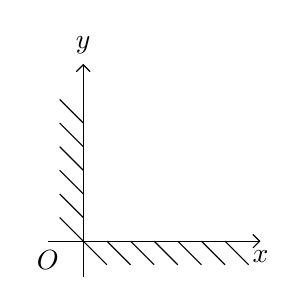
\begin{tikzpicture}[scale=1.5]
\draw[<-,>=angle 90] (1.5,0)node[below]{$x$} -- (-0.3,0) node[below] {$O$};
\draw[->,>=angle 90] (0,-0.3)   -- (0,1.5) node[above] {$y$};
\draw (0,0) -- (0.2,-0.2);
\draw (0.2,0) -- (0.4, -0.2); 
\draw (0.4,0) -- (0.6,-0.2);
\draw (0.6,0) -- (0.8, -0.2); 
\draw (0.8,0) -- (1,-0.2);
\draw (1,0) -- (1.2, -0.2); 
\draw (1.2,0) -- (1.4,-0.2);
\draw (0,0) -- (-0.2, 0.2);
\draw (0,0.2) -- (-0.2, 0.4);
\draw (0,0.4) -- (-0.2, 0.6);
\draw (0,0.6) -- (-0.2, 0.8);
\draw (0,0.8) -- (-0.2, 1);
\draw (0,1) -- (-0.2, 1.2);
\end{tikzpicture}
\end{center}
最后, 作映射$ w = \eta^2$. 由幂函数的性质可得, 它将$\eta$平面的第一象限映射为$w$平面的上半平面. 

完整的图示如下:
\begin{center}
\begin{tikzpicture}[scale=1.5]
\draw[<-,>=angle 90] (1.5,0)node[below]{$x$} -- (-0.3,0) node[below] {$O$};
\draw[->,>=angle 90] (0,-0.3)   -- (0,1.5) node[above] {$y$};
\draw plot[domain=0:1] (\x,{(1 -\x^2)^0.5}) ;
\fill (1,0) node[below]{$1$};
\fill (0.5, 0.6) node[below]{$D$};
\fill (0,1) node[left]{$1$};
\draw[->, >=angle 90] (1.6, 0.6) -- (2.6, 0.6);
\fill (2.1, 0.6) node[above]{$ \xi = z^2$};
\draw[->, >=angle 90] (2.7, 0) -- (5.3, 0) node[below]{$x$};
\draw[->, >=angle 90] (4, -0.3) -- (4, 1.5) node[above]{$y$};
\draw plot[domain=3:5] (\x, {(1-(\x-4)^2)^0.5});
\draw[->, >=angle 90] (4, -0.4) -- (4, -1.2);
\fill (4, -0.8) node[right]{$\eta = \dfrac{1+\xi}{1-\xi}$};
\end{tikzpicture} 
\end{center}
\begin{center}
\begin{tikzpicture}[scale=1.5]
\draw[<-,>=angle 90] (2.5,0)node[below]{$x$} -- (-0.3,0);
\fill (0.9,0) node[above]{$O$};
\draw[->,>=angle 90] (1,-0.3)   -- (1,2) node[above] {$y$};
\draw (0, 0) -- (-0.2, -0.2);
\draw (0.2, 0) -- (0, -0.2);
\draw (0.4, 0) -- (0.2, -0.2);
\draw (0.6, 0) -- (0.4, -0.2);
\draw (0.8, 0) -- (0.6, -0.2);
\draw (1, 0) -- (0.8, -0.2);
\draw (1.2, 0) -- (1, -0.2);
\draw (1.4, 0) -- (1.2, -0.2);
\draw (1.6, 0) -- (1.4, -0.2);
\draw (1.8, 0) -- (1.6, -0.2);
\draw (2, 0) -- (1.8, -0.2);
\draw (2.2, 0) -- (2, -0.2);
\draw[<-,>=angle 90] (2.7,0.8)   -- (3.7,0.8);
\fill (3.2, 0.8) node[above]{$w = \eta^2$};
\end{tikzpicture}  
\begin{tikzpicture}[scale=1.5]
\draw[<-,>=angle 90] (1.8,0)node[below]{$x$} -- (-0.3,0) node[below] {$O$};
\draw[->,>=angle 90] (0,-0.3)   -- (0,2) node[above] {$y$};
\draw (0,0) -- (0.2,-0.2);
\draw (0.2,0) -- (0.4, -0.2); 
\draw (0.4,0) -- (0.6,-0.2);
\draw (0.6,0) -- (0.8, -0.2); 
\draw (0.8,0) -- (1,-0.2);
\draw (1,0) -- (1.2, -0.2); 
\draw (1.2,0) -- (1.4,-0.2);
\draw (0,0) -- (-0.2, 0.2);
\draw (0,0.2) -- (-0.2, 0.4);
\draw (0,0.4) -- (-0.2, 0.6);
\draw (0,0.6) -- (-0.2, 0.8);
\draw (0,0.8) -- (-0.2, 1);
\draw (0,1) -- (-0.2, 1.2);
\draw (0,1.2) -- (-0.2, 1.4);
\draw (0,1.4) -- (-0.2, 1.6);
\draw (0,1.6) -- (-0.2, 1.8);
\end{tikzpicture} 
\end{center}
将以上映射复合起来, 可以得到:
$$ w = \dfrac{(1+z^2)^2}{(1-z^2)^2} = \dfrac{z^4 + 2z^2 + 1}{z^4 - 2z^2 + 1} $$ 

\newpage

\section{2014-2015学年第二学期复变函数期末考试(12级)}
\textbf{一、(本题48分, 每小题8分)}

(1) 求$cos(\dfrac{\pi}{4} + i)$.

\textbf{解:} 
$$ cos(\dfrac{\pi}{4}+i) = \dfrac{e^{i(\frac{\pi}{4} + i)} + e^{-i(\frac{\pi}{4} + i)}}{2} = \dfrac{e^{-1 + i\frac{\pi}{4}} + e^{1-i\frac{\pi}{4}}}{2} = \dfrac{\sqrt{2}}{4}(e + \dfrac{1}{e}) + i\dfrac{\sqrt{2}}{4} (\dfrac{1}{e} - e) $$ \\ 

(2) 讨论$f(z) = x^2 + 2xy - y^2 + i(ax^2 + 2xy + y^2)$的可导性、解析性. 

\textbf{证明:} 

记$u(x,y) = x^2 + 2xy - y^2$, $v(x,y) = ax^2 + 2xy + y^2$. 则:
$$ \dfrac{\partial u}{\partial x} = 2x + 2y, \ \dfrac{\partial u}{\partial y} = 2x - 2y, \ \dfrac{\partial v}{\partial x} = 2ax + 2y, \ \dfrac{\partial v}{\partial y} = 2x + 2y$$
注意到: $\dfrac{\partial u}{\partial x} = \dfrac{\partial v}{\partial y} = 2x + 2y$成立. 下面分情况讨论:

(i) 当$a =-1$时, $\dfrac{\partial u}{\partial y} = -\dfrac{\partial v}{\partial x}$. 由于$u,v$在复平面有连续的一阶偏导数, 并且处处满足C-R条件. 所以$f(z)$在复平面上解析, 在复平面处处可导. 

(ii) 当$a \neq -1$时, C-R条件仅仅在直线$x=0$上满足. 由于$u,v$在复平面有连续的一阶偏导数, 所以$f(z)$在直线$x=0$上可导, 在复平面上处处不解析. \\  \\  


(3)求$I = \displaystyle{\int_L \dfrac{zsinz}{(z+1)^2(z-1)}dz}$, $L$分别为$|z|=\dfrac{1}{2}, |z-1|=\dfrac{1}{2}$以及$|z+1|=\dfrac{1}{2}$. 

\textbf{证明:} 

(i) 由于$f(z) =\dfrac{zsinz}{(z+1)^2(z-1)}dz $在$|z|<\dfrac{1}{2}$内无奇点, 在$|z| \leq \dfrac{1}{2}$上连续, 由Cauchy积分定理可知:
$$ I = \displaystyle{\int_{L_1} \dfrac{zsinz}{(z+1)^2(z-1)}dz} = 0 $$
(ii) 由于$f_2(z) = \dfrac{zsinz}{(z+1)^2}$在$|z-1| \leq \dfrac{1}{2}$上解析, 由Cauchy积分公式:
$$ I = \displaystyle{\int_{L_2} \dfrac{zsinz}{(z+1)^2(z-1)}dz} = \displaystyle{\int_{L_2} \dfrac{f_2(z)}{z-1}dz} = 2\pi i f_2(1) = \dfrac{\pi i sin1}{2}$$
(iii) 由于$f_3(z) = \dfrac{zsinz}{z-1}$在$|z+1| \leq \dfrac{1}{2}$上解析, 由Cauchy导数公式:
$$ \displaystyle{\int_{L_3} \dfrac{zsinz}{(z+1)^2(z-1)}dz} = \displaystyle{\int_{L_3} \dfrac{f_3(z)}{(z+1)^2}dz} = 2\pi i f_3'(z)|_{z=-1} = \dfrac{\left(sin1 + 2cos1 \right)\pi i}{2} $$ \\ 

(4) $f(z)$是整函数, $Re f(z) \leq M$. 证明$f(z) = $常数. 

\textbf{证明:}  

考虑函数$g(z) = e^{f(z)}$. 由10年第(6)题证明过程可知: $g(z)$在$C$上解析. 所以$g(z)$也是整函数. 而:
$$ |g(z)| = |e^{f(z)}| = |e^{u+iv}| = e^u = e^{Re f(z)} \leq e^M $$
所以$g(z)$是有界整函数, 由刘维尔定理可知, $g(z) = e^{f(z)} = $常数. 从而:
$$ g'(z) = f'(z)e^f(z) = 0 \ \ \Rightarrow \ \ f'(z) = 0 $$ 
从而: f(z)在$\mathbb{C}$上为常数. \\  \\



(5) 证明$a>e$时, $e^{z^2} = az^n$在$|z|<1$内有$n$个根. 

\textbf{证明:}

由09年第(4)题可知:$\forall z \in \mathbb{C}$
$$ |e^z| \leq e^{|z|} $$
记$f(z) = az^n, g(z) = -e^{z^2}$, 则在$|z| = 1$上:
$$ |-g(z)| = |e^{z^2}| \leq e^{|z^2|}  = e < |a| = |az^n| = |f(z)|$$
由于$f(z), g(z)$在$|z|\leq 1$上解析, 由Rouche定理可知, 
$$ f(z)=az^n, \ \ f(z) + g(z) = az^n - e^{z^2} $$
在$|z|<1$内有相同个数的零点. 而$f(z)$在$|z|<1$内有n重零点$z=0$, 所以$az^n = e^{z^2}$在$|z|<1$内有n个根.\\  \\ 

(6) $f(z) = e^{z-\frac{1}{z}} $, 判断$z=0$的奇点类型, 并求Res$(f,0)$.


\textbf{解:} 

取$x_n = \dfrac{1}{n} $, $y_n = -\dfrac{1}{n}$, 则$x_n \rightarrow 0, y_n \rightarrow 0$. 而:
$$ \lim\limits_{n \rightarrow +\infty} f(x_n) = \lim\limits_{n \rightarrow +\infty} e^{\frac{1}{n}-n} = 0, \ \ \lim\limits_{n \rightarrow +\infty} f(y_n) = \lim\limits_{n \rightarrow +\infty} e^{-\frac{1}{n}+n} = + \infty $$
所以$f(z)$在$z=0$不存在有限或无穷的极限. 而$f(z)$在$0<|z|<R$内解析, 所以$z=0$是$f(z)$的本性奇点.

下求Res$(f,0)$. 只需要求$f$在$z=0$处展开的洛朗级数中$\dfrac{1}{z}$的系数.

$$ f(z) = e^{z-\frac{1}{z}} = e^ze^{-\frac{1}{z}} = \left( \sum\limits_{n=0}^{+\infty} \dfrac{1}{n!} z^n \right)\left(\sum\limits_{n=0}^{+\infty} \dfrac{(-1)^n}{n!} \dfrac{1}{z^n}  \right) $$
由排列组合的相关知识点可知,
$$ \text{Res}(f, 0) = \alpha_{-1} = \sum\limits_{n=0}^{+\infty} \dfrac{1}{n!} \dfrac{(-1)^{n+1}}{(n+1)!} = \sum\limits_{n=0}^{+\infty} \dfrac{(-1)^{n+1}}{n!(n+1)!}  $$ \\ 

\textbf{二、(本题10分)}

设$f(z)$在$0<|z-z_0|<R$内解析, 且有界. 证明对于$\forall 0<r<R$, 有:
$$  \int_{|z-z_0|=r} f(z) dz = 0 $$
提示: 说明对$\forall 0< \epsilon < r$, $\int_{|z-z_0|=r} f(z) dz = \int_{|z-z_0|=\epsilon} f(z)dz$. 

\textbf{证明:}  

首先, 对于$\forall 0<\epsilon<r$, 作圆环$D = \{z: \epsilon<|z-z_0|<r  \}$, 则$f(z)$在$D$上解析, 且(积分路径取逆时针):
$$ \int_{|z-z_0|=r} f(z) dz = \int_{|z-z_0|=\epsilon} f(z) dz  $$
由于$f(z)$在$0<|z-z_0|<R$内有界, 所以存在$M$>0, 使得$|f(z)| \leq M$. 而:
$$ \left| \int_{|z-z_0|=\epsilon} f(z) dz \right| \leq \int_{|z-z_0|=\epsilon} \left| f(z) \right| \left| dz \right| \leq 2M\pi \epsilon \rightarrow 0  $$
所以:
$$  \int_{|z-z_0|=r} f(z) dz =  \lim\limits_{\epsilon \rightarrow 0} \int_{|z-z_0|=\epsilon} f(z) dz = 0  $$ \\  

\textbf{三、(本题10分)}

设$D$是有界区域, $f(z)$在$D$内解析, 在$\overline{D}$上连续, 在$D$内无零点. 证明:若在边界$L$上$f(z) \equiv $常数, 则在$D$内$f(z) \equiv $常数. 

提示: 对$f(z)$和$\dfrac{1}{f(z)}$用最大模原理. 

\textbf{证明:} 

由于$f(z)$在$D$内解析, 在$\overline{D}$上连续, 在$D$内无零点, 所以$\dfrac{1}{f(z)}$也在$D$内解析, 在$\overline{D}$上连续.

假设$f(z)$在$D$内不恒为常数. 由最大模原理的推论, $|f(z)|$, $\left|\dfrac{1}{f(z)}\right|$都在$D$的边界$L$上达到最大值.

而在边界$L$上, $f(z) = C$. 所以, 在$D$内:
$$ |f(x)| < C, \ \ \left| \dfrac{1}{f(z)} \right| < \dfrac{1}{C} \ \ \Rightarrow \ \ |f(z)|<C, |f(z)|>C  $$
矛盾. 所以$f(z)$在$D$内恒为常数. \\  \\


\textbf{四、(本题12分)}

确定$F(z) = \sqrt[3]{z^2(z-1)}$的枝点, 作出$F(z)$的可单值分枝区域$D$, 使得$D$中包含$2$和$i$. $f(z)$是$F(z)$在$z=2$时取正值的单值解析分枝. 求$f(i)$. 

\textbf{解:} 

由于$2,1$不是$3$的倍数, $2+1$是$3$的倍数, 所以$0,1$是$F(z)$的枝点, $\infty$不是$F(z)$的枝点. 根据根式函数的定义:
$$ F(z) = \sqrt[3]{|z^2(z-1)|} e^{i\dfrac{2Argz + Arg(z-1)}{3}} $$
以区间$[0,1]$为割线割开复平面$\mathbb{C}$得到区域$D$, 下说明$D$是$F(z)$的可单值分枝区域. 对于$D$内任意一条简单封闭曲线$L$, $L$或者不围绕$0,1$, 或者同时围绕$0,1$. 设$z_0$是$L$上任意一点, 当$z_0$沿着$L$逆时针运动回到$z_0$时, 或者$argz, arg(z-1)$都不变, 或者$argz, arg(z-1)$同时增加$2\pi$, 两种情况下$F(z)$都不发生改变. 所以$D$确实是$F(z)$的一个可单值分枝区域. 注意到$2$和$i$在区域$D$内, 所以我们所作的区域$D$符合题目要求.

下面计算指定单值分枝在给定点的函数值. 在$z=2$处, 取:
$$ argz = 0, \ \ arg(z-1) = 0 $$
所以:
$$ f(2) = \sqrt[3]{4} e^{i\dfrac{2k\pi}{3}} = \sqrt[3]{2}\left[cos(\dfrac{2\pi}{3}) + isin(\dfrac{2\pi}{3}) \right] $$
由于$f(2)$取正值, 所以$k=0$. 从而:
$$ f(i) = \sqrt[6]{2} e^{i\dfrac{2\times \frac{\pi}{2} + \frac{3\pi}{4}}{3}} = \sqrt[6]{2}\left[cos(\dfrac{7\pi}{12}) + isin(\dfrac{7\pi}{12})  \right] $$ \\ 


\textbf{五、(本题10分)}

用留数定理求积分$I = \displaystyle{\int_0^{+\infty} \dfrac{sinx}{x(x^2+1)}dx}$.

\textbf{解:}

令$g(z) = \dfrac{e^{iz}}{z(z^2+1)}$, 则$g(z)$在上半平面除了有一个一阶极点$z=i$以及在积分路径上有一个一阶奇点$z=0$外处处解析. 设$D$是以$O$为圆心,$R$为半径的上半圆盘. 当$R>1$时, $z=i$在区域$D$中. 设$D$的边界由$C_R + L_R$组成, 由留数定理可知:
\begin{align*}
 \displaystyle{\int_{-R}^{R} \dfrac{e^{ix}}{x(x^2+1)}dx} + \displaystyle{\int_{C_R} \dfrac{e^{iz}}{z(z^2+1)}dz} &= 2\pi i \left(\text{Rex}(f,i) + \dfrac{1}{2}\text{Res}(f,0)\right) \\
    &= 2\pi i \left( \left.\dfrac{e^{iz}}{z(z+i)} \right|_{z=i} +  \left. \dfrac{1}{2} \dfrac{e^{iz}}{z^2+1} \right|_{z=0} \right) \\
    &= \left(1-\dfrac{1}{e} \right)\pi i 
\end{align*}
由于$\lim\limits_{z \rightarrow \infty} \dfrac{1}{z(z^2+1)} = 0$, 所以:
$$ \lim\limits_{R \rightarrow +\infty} \displaystyle{\int_{C_R} \dfrac{e^{iz}}{z(z^2 + 1)}dz} = 0 $$
令$R \rightarrow +\infty$,有:
$$\displaystyle{\int_{-\infty}^{+\infty} \dfrac{e^{ix}}{x(x^2+1)}dx} = \displaystyle{\int_{-\infty}^{+\infty} \dfrac{cosx}{x(x^2+1)}dx} + \displaystyle{\int_{-\infty}^{+\infty} \dfrac{isinx}{x(x^2+1)}dx}=\left(1 -\dfrac{1}{e}\right)\pi i $$
比较实部虚部,及结合$\dfrac{sinx}{x(x^2+1)}$是个偶函数可得:
$$ I = \displaystyle{\int_0^{+\infty} \dfrac{sinx}{x(x^2+1)}dx} = \dfrac{1}{2}\displaystyle{\int_{-\infty}^{+\infty} \dfrac{sinx}{x(x^2+1)}dx} = \dfrac{\pi}{2}\left(1 - \dfrac{1}{e}\right) $$  

\textbf{另解:}

令$g(z) = \dfrac{e^{iz}}{z(z^2+1)}$. 作如下图所示的积分路径:
\begin{center}
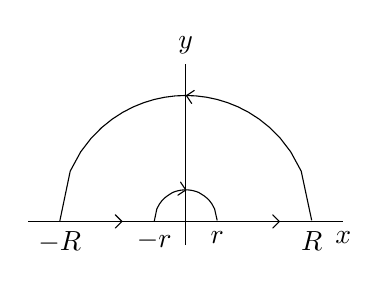
\begin{tikzpicture}
\draw (-2, 0) -- (2, 0) node[below]{$x$};
\draw (0, -0.3) -- (0, 2) node[above]{$y$};
\draw plot[domain=-1.6:1.6] (\x, {(1.6^2-(\x)^2)^0.5});
\draw plot[domain=-0.4:0.4] (\x, {(0.4^2-(\x)^2)^0.5});
\fill (-0.4, 0) node[below]{$-r$};
\fill (0.4, 0) node[below]{$r$};
\fill (-1.6, 0) node[below]{$-R$};
\fill (1.6,0) node[below]{$R$};
\draw[->, >=angle 90] (-1.2, 0) -- (-0.8, 0);
\draw[->, >=angle 90] (0.8, 0) -- (1.2, 0);
\draw[->, >=angle 90] (0.01, 1.598) -- (0, 1.6);
\draw[<-, >=angle 90] (0.01, 0.398) -- (0, 0.4);
\end{tikzpicture}
\end{center}
当$g(z)$沿着如上图所示的路径积分时, 它在以该路径为边界的区域内只有一个一阶极点$z=i$. 由留数定理可知:
$$
\int_{-R}^{-r} \dfrac{e^{ix}}{x(x^2+1)}dx + \int_{C_r^-} \dfrac{e^{iz}}{z(z^2+1)}dz + \int_{r}^{R} \dfrac{e^{ix}}{x(x^2+1)}dx + \int_{C_R} \dfrac{e^{iz}}{z(z^2+1)}dz = 2\pi i \text{Res}(g, i)  = -\dfrac{\pi i }{e}
$$
当$R \rightarrow +\infty$时, 由于$\lim\limits_{z \rightarrow \infty} \dfrac{1}{z(z^2 + 1)} = 0$, 所以:
$$ \lim\limits_{R \rightarrow +\infty} \int_{C_R} \dfrac{e^{iz}}{z(z^2+1)}dz = 0  $$
又由于:
$$ \lim\limits_{z \rightarrow 0} zg(z) = \lim\limits_{z=0} \dfrac{e^{iz}}{z^2 + 1} = 1 $$
所以:
$$ \lim\limits_{r \rightarrow} \int_{C_r^-} \dfrac{e^{iz}}{z(z^2+1)}dz = -i \times (\pi -0) = -\pi i  $$
令$R \rightarrow +\infty, r \rightarrow 0$, 有:
$$ \int_{-\infty}^{+\infty} \dfrac{e^{ix}}{x(x^2 + 1)}dx = \int_{-\infty}^{+\infty} \dfrac{cosx}{x(x^2 + 1)}dx + \int_{-\infty}^{+\infty} \dfrac{isinx}{x(x^2 + 1)}dx= -\dfrac{\pi i }{e} + \pi i = (1 - \dfrac{1}{e})\pi i $$
比较实部虚部以及结合$\dfrac{sinx}{x(x^2 + 1)}$是偶函数可得:
$$ I = \displaystyle{\int_0^{+\infty} \dfrac{sinx}{x(x^2+1)}dx} = \dfrac{1}{2}\displaystyle{\int_{-\infty}^{+\infty} \dfrac{sinx}{x(x^2+1)}dx}  = \dfrac{\pi}{2}(1-\dfrac{1}{e}) $$ \\ 



\textbf{六、(本题10分)}

作保形映射将$D = \{ z: |z|<1 , Re f(z) > 0\}$(如下图)映射为$|w|<1$.
\begin{center}
\begin{tikzpicture}[scale=1.5]
\draw[->, >=angle 90] (-0.3, 0) -- (1.5, 0) node[below]{$x$};
\draw[->, >=angle 90] (0,-1.5) -- (0,1.5) node[above]{$y$};
\draw plot[domain=0:1] (\x, {(1-\x^2)^0.5});
\draw plot[domain=0:1] (\x, {-(1-\x^2)^0.5});
\fill (1.1, 0) node[below]{$1$};
\fill (-0.1,0) node[below]{$O$};
\fill (0,1) node[left]{$i$};
\fill (0,-1) node[left]{$-i$};
\end{tikzpicture}
\end{center}

提示: 先作映射$\xi = \dfrac{z+i}{z-i}$.

\textbf{解:}

先作映射$\xi = \dfrac{z+i}{z_i}$. 映射$\xi$将$z$平面上的$-i, 0, i$映射为$\xi$平面上的$0, -1, \infty$. 由分式线性映射的保圆性可知, $\xi$把$z$平面上的虚轴映射为负半实轴; $\xi$还将$z$平面圆弧上的点$-i, 1, i$映射为$0, i, \infty$, 由分式线性映射的保圆性可知, $\xi$将圆弧映射为正半虚轴. 取区域$D$内的点$z=\dfrac{1}{2}$, 则$\xi$将$z=\dfrac{1}{2}$映射为$\xi = -\dfrac{3}{5} + i\dfrac{4}{5}$, 在第二象限. 所以映射$\xi$将$z$平面的区域$D$映射为$\xi$平面的第二象限. 
\begin{center}
\begin{tikzpicture}[scale=1.5]
\draw[->, >=angle 90] (-0.3, 0) -- (1.5, 0) node[below]{$x$};
\draw[->, >=angle 90] (0,-1.5) -- (0,1.5) node[above]{$y$};
\draw plot[domain=0:1] (\x, {(1-\x^2)^0.5});
\draw plot[domain=0:1] (\x, {-(1-\x^2)^0.5});
\fill (1.1, 0) node[below]{$1$};
\fill (-0.1,0) node[below]{$O$};
\fill (0,1) node[left]{$i$};
\fill (0,-1) node[left]{$-i$};
\draw[->, >=angle 90] (1.7, 0) -- (2.7, 0);
\fill (2.2, 0) node[above]{$\xi = \dfrac{z+i}{z-i}$};
\draw[->, >=angle 90] (2.9, -0.6) -- (5.5, -0.6) node[below]{$x$};
\draw[->, >=angle 90] (5, -1.3) -- (5, 1.5) node[left]{$y$};
\fill (5.2, -0.6) node[below]{$O$};
\draw (5, -0.6) -- (4.8, -0.8);
\draw (4.8, -0.6) -- (4.6, -0.8);
\draw (4.6, -0.6) -- (4.4, -0.8);
\draw (4.4, -0.6) -- (4.2, -0.8);
\draw (4.2, -0.6) -- (4, -0.8);
\draw (4, -0.6) -- (3.8, -0.8);
\draw (3.8, -0.6) -- (3.6, -0.8);
\draw (3.6, -0.6) -- (3.4, -0.8);
\draw (3.4, -0.6) -- (3.2, -0.8);
\draw (3.2, -0.6) -- (3, -0.8);
\draw (5, -0.6) -- (5.2, -0.4);
\draw (5, -0.4) -- (5.2, -0.2);
\draw (5, -0.2) -- (5.2, 0);
\draw (5, 0) -- (5.2, 0.2);
\draw (5, 0.2) -- (5.2, 0.4);
\draw (5, 0.4) -- (5.2, 0.6);
\draw (5, 0.6) -- (5.2, 0.8);
\draw (5, 0.8) -- (5.2, 1);
\draw (5, 1) -- (5.2, 1.2);
\draw[->, >=angle 90] (5.2, -1.5) -- (6, -2.4);
\fill (5.7, -2) node[right]{$\eta = e^{-i\frac{\pi}{2}} \xi = -i \xi$};
\end{tikzpicture}
\end{center}
\begin{center}
\begin{tikzpicture}[scale = 1.3]
\draw[->, >=angle 90] (-1.5, 0) -- (1.5, 0) node[below]{$x$};
\draw[->, >=angle 90] (0,-1.5) -- (0,1.5) node[above]{$y$};
\draw plot[domain=-1:1] (\x, {(1-(\x)^2)^0.5});
\draw plot[domain=-1:1] (\x, {-(1-(\x)^2)^0.5});
\fill (1.1, 0) node[below]{$1$};
\fill (-0.1,0) node[below]{$O$};
\fill (0,1.1) node[left]{$i$};
\fill (0,-1.1) node[left]{$-i$};
\draw[<-, >=angle 90] (1.7, 0) -- (2.7, 0);
\fill (2.2, 0) node[above]{$w = \dfrac{\beta-i}{\beta+i}$};
\end{tikzpicture}
\begin{tikzpicture}[scale=1.3]
\draw[->, >=angle 90] (-1.5, -0.5) -- (1.5, -0.5) node[below]{$x$};
\draw[->, >=angle 90] (0,-1.5) -- (0,1.5) node[above]{$y$};
\fill (-0.2, -0.5) node[above]{$O$};
\draw (-1.2, -0.5) -- (-1, -0.7);
\draw (-1, -0.5) -- (-0.8, -0.7);
\draw (-0.8, -0.5) -- (-0.6, -0.7);
\draw (-0.6, -0.5) -- (-0.4, -0.7);
\draw (-0.4, -0.5) -- (-0.2, -0.7);
\draw (-0.2, -0.5) -- (0, -0.7);
\draw (0, -0.5) -- (0.2, -0.7);
\draw (0.2, -0.5) -- (0.4, -0.7);
\draw (0.4, -0.5) -- (0.6, -0.7);
\draw (0.6, -0.5) -- (0.8, -0.7);
\draw (0.8, -0.5) -- (1, -0.7);
\draw (1, -0.5) -- (1.2, -0.7);
\draw[<-, >=angle 90] (1.7, 0) -- (2.7, 0);
\fill (2.2, 0) node[above]{$\beta = \eta^2$};
\end{tikzpicture}
\begin{tikzpicture}[scale=1.3]
\draw[->, >=angle 90] (-1.5, -0.5) -- (1.5, -0.5) node[below]{$x$};
\draw[->, >=angle 90] (-0.8,-1.5) -- (-0.8,1.5) node[above]{$y$};
\fill (-1, -0.5) node[below]{$O$};
\draw (-0.8, -0.5) -- (-0.6, -0.7);
\draw (-0.6, -0.5) -- (-0.4, -0.7);
\draw (-0.4, -0.5) -- (-0.2, -0.7);
\draw (-0.2, -0.5) -- (0, -0.7);
\draw (0, -0.5) -- (0.2, -0.7);
\draw (0.2, -0.5) -- (0.4, -0.7);
\draw (0.4, -0.5) -- (0.6, -0.7);
\draw (0.6, -0.5) -- (0.8, -0.7);
\draw (0.8, -0.5) -- (1, -0.7);
\draw (1, -0.5) -- (1.2, -0.7);
\draw (-0.8, -0.5) -- (-1, -0.3);
\draw (-0.8, -0.3) -- (-1, -0.1);
\draw (-0.8, -0.1) -- (-1, 0.1);
\draw (-0.8, 0.1) -- (-1, 0.3);
\draw (-0.8, 0.3) -- (-1, 0.5);
\draw (-0.8, 0.5) -- (-1, 0.7);
\draw (-0.8, 0.7) -- (-1, 0.9);
\draw (-0.8, 0.9) -- (-1, 1.1);
\draw (-0.8, 1.1) -- (-1, 1.3);
\end{tikzpicture}
\end{center}
再作映射$\eta = e^{-i\frac{\pi}{2}}\xi$, 这个映射是旋转变换(顺时针旋转$\dfrac{\pi}{2}$), 将第二象限映射为第一象限. 

再作映射$\beta = \eta^2$, 这个映射将第一象限张成上半平面. 

最后取$\beta$平面关于实轴对称的两点$i, -1$, 作映射:
$$ w = \dfrac{\beta - i}{\beta + i} $$
它把$\beta$平面的上半圆盘映射为$w$平面的单位圆$|w| < 1$.将上述映射复合起来, 可得:
$$ w = \dfrac{(z+i)^2 + i(z-i)^2}{(z+i)^2 - i(z-i)^2} = \dfrac{(1+i)z^2 + 2(1+i)z -(1+i)}{(1-i)z^2 -2(1-i)z - (1-i)} = i \dfrac{z^2 + 2z - 1}{z^2 - 2z - 1} $$






\end{document} 